%%%%%%%%%%%%%%%%%%%%%%%%%%%%%%%%%%%%%%%%%%%%%%%%%%%%%%%%%%%%%%%%%%%%%%%%%%%%
% AGUtmpl.tex: this template file is for articles formatted with LaTeX2e,
% Modified March 2013
%
% This template includes commands and instructions
% given in the order necessary to produce a final output that will
% satisfy AGU requirements.
%
% PLEASE DO NOT USE YOUR OWN MACROS
% DO NOT USE \newcommand, \renewcommand, or \def.
%
% FOR FIGURES, DO NOT USE \psfrag or \subfigure.
%
%%%%%%%%%%%%%%%%%%%%%%%%%%%%%%%%%%%%%%%%%%%%%%%%%%%%%%%%%%%%%%%%%%%%%%%%%%%%
%
% All questions should be e-mailed to latex@agu.org.
%
%%%%%%%%%%%%%%%%%%%%%%%%%%%%%%%%%%%%%%%%%%%%%%%%%%%%%%%%%%%%%%%%%%%%%%%%%%%%
%
% Step 1: Set the \documentclass
%
% There are two options for article format: two column (default)
% and draft.
%
% PLEASE USE THE DRAFT OPTION TO SUBMIT YOUR PAPERS.
% The draft option produces double spaced output.
%
% Choose the journal abbreviation for the journal you are
% submitting to:

% jgrga JOURNAL OF GEOPHYSICAL RESEARCH
% gbc   GLOBAL BIOCHEMICAL CYCLES
% grl   GEOPHYSICAL RESEARCH LETTERS
% pal   PALEOCEANOGRAPHY
% ras   RADIO SCIENCE
% rog   REVIEWS OF GEOPHYSICS
% tec   TECTONICS
% wrr   WATER RESOURCES RESEARCH
% gc    GEOCHEMISTRY, GEOPHYSICS, GEOSYSTEMS
% sw    SPACE WEATHER
% ms    JAMES
% ef    EARTH'S FUTURE
%
%
%
% (If you are submitting to a journal other than jgrga,
% substitute the initials of the journal for "jgrga" below.)

\documentclass[jgrga, draft]{agutex}
% \documentclass[jgrga]{agutex}
% To create numbered lines:

% If you don't already have lineno.sty, you can download it from
% http://www.ctan.org/tex-archive/macros/latex/contrib/ednotes/
% (or search the internet for lineno.sty ctan), available at TeX Archive Network (CTAN).
% Take care that you always use the latest version.

% To activate the commands, uncomment \usepackage{lineno}
% and \linenumbers*[1]command, below:

\usepackage{lineno}
\linenumbers*[1]

%  To add line numbers to lines with equations:
%  \begin{linenomath*}
%  \begin{equation}
%  \end{equation}
%  \end{linenomath*}
\usepackage{amsmath}

\usepackage{enumitem}
% \usepackage{hyperref}
%%%%%%%%%%%%%%%%%%%%%%%%%%%%%%%%%%%%%%%%%%%%%%%%%%%%%%%%%%%%%%%%%%%%%%%%%
% Figures and Tables
%
%
% DO NOT USE \psfrag or \subfigure commands.
%
%  Figures and tables should be placed AT THE END OF THE ARTICLE,
%  after the references.
%
%  Uncomment the following command to include .eps files
 % \usepackage[pdflatex]{graphicx}
 \usepackage{graphicx}
 \DeclareGraphicsExtensions{.pdf, .png, .jpg, .eps}
 \graphicspath{ {./figs/} }

%
%  Uncomment the following command to allow illustrations to print
%   when using Draft:
 \setkeys{Gin}{draft=false}
%
% Substitute one of the following for [dvips] above
% if you are using a different driver program and want to
% proof your illustrations on your machine:
%
% [xdvi], [dvipdf], [dvipsone], [dviwindo], [emtex], [dviwin],
% [pctexps],  [pctexwin],  [pctexhp],  [pctex32], [truetex], [tcidvi],
% [oztex], [textures]
%
% See how to enter figures and tables at the end of the article, after
% references.
%
%% ------------------------------------------------------------------------ %%
%
%  ENTER PREAMBLE
%
%% ------------------------------------------------------------------------ %%

% Author names in capital letters:
\authorrunninghead{HAMMAN ET AL.}

% Shorter version of title entered in capital letters:
\titlerunninghead{COASTAL STREAMFLOW FLUX IN RASM}

%Corresponding author mailing address and e-mail address:
\authoraddr{Corresponding author: Bart Nijssen,
Department of Civil \& Environmental Engineering, Box 352700,
University of Washington, Seattle, WA 98195-2700, USA.
(nijssen@uw.edu)}

\begin{document}

%% ------------------------------------------------------------------------ %%
%
%  TITLE
%
%% ------------------------------------------------------------------------ %%


\title{The Coastal Streamflow Flux in the Regional Arctic System Model}

% Could use another title, TBD. WM

%% ------------------------------------------------------------------------ %%
%
%  AUTHORS AND AFFILIATIONS
%
%% ------------------------------------------------------------------------ %%


% Use \author{\altaffilmark{}} and \altaffiltext{}

% \altaffilmark will produce footnote;
% matching \altaffiltext will appear at bottom of page.

\authors{Joseph Hamman\altaffilmark{1,4},
Bart Nijssen\altaffilmark{1},
Andrew Roberts\altaffilmark{2},
Anthony Craig\altaffilmark{2},
Wieslaw Maslowski\altaffilmark{2},
and Robert Osinski\altaffilmark{3}}

\altaffiltext{1}{Department of Civil \& Environmental Engineering,
University of Washington, Seattle, WA, USA.}
\altaffiltext{2}{Department of Oceanography, Naval Postgraduate School,
Monterey, CA, USA.}
\altaffiltext{3}{Polish Institute of Oceanology, Sopot, Poland.}
\altaffiltext{4}{National Center for Atmospheric Research, Boulder, Colorado, USA.}


%% ------------------------------------------------------------------------ %%
%
%  ABSTRACT
%
%% ------------------------------------------------------------------------ %%

% >> Do NOT include any \begin...\end commands within
% >> the body of the abstract.
% The purpose of the abstract is twofold: (1) state the nature of the investigation and (2) summarize the important conclusions of this investigation. The abstract should be suitable for separate publication in an abstract journal and be adequate for indexing. Make sure to check for the following:
%
% It is set as a single paragraph.
% It is limited to 250 words for all journals except GRL where the limit is 150 words.
% It does not include table or figure mentions.
% If it has reference citations that are part of the sentence, they should be in roman type and have parentheses around the year; parenthetical reference citations will be deleted.
% All abbreviations used in the abstract are defined.

\begin{abstract}
The coastal streamflow flux from the Arctic drainage basin is an important driver of dynamics in the coupled ice-ocean system.
Comprising more than one-third of the total freshwater flux into the Arctic Ocean, streamflow is a key component of the regional and global freshwater cycle.
To better represent the coupling of the streamflow flux to the ocean, we have developed and applied the RVIC streamflow routing model within the Regional Arctic System Model (RASM).
The RASM is a high-resolution regional Earth System Model whose domain includes all of the Arctic drainage basin.
In this paper, we introduce the RVIC streamflow routing model, detailing its application within RASM and its advancements in terms of representing high-resolution streamflow processes.
We evaluate model simulated streamflow relative to in-situ observations and demonstrate a method for improving model performance using a simple optimization procedure.
We also present a new, spatially and temporally consistent, high-resolution dataset of coastal freshwater fluxes for the Arctic drainage basin and surrounding areas that is based on a fully-coupled RASM simulation and intended for use in Arctic Ocean modeling applications.
This dataset is evaluated relative to other coastal streamflow datasets commonly used by the ocean modeling community.
We demonstrate that the RASM-simulated streamflow flux better represents the annual cycle than existing datasets, especially in ungauged areas.
Finally, we assess the impact that streamflow has on the coupled ice-ocean system, finding that the presence of streamflow leads to reduced sea surface salinity, increased sea surface temperatures, and decreased sea ice thickness.

\end{abstract}

%% ------------------------------------------------------------------------ %%
%
%  BEGIN ARTICLE
%
%% ------------------------------------------------------------------------ %%

% The body of the article must start with a \begin{article} command
%
% \end{article} must follow the references section, before the figures
%  and tables.

\begin{article}

%% ------------------------------------------------------------------------ %%
%
%  TEXT
%
%% ------------------------------------------------------------------------ %%

\section{Introduction}
\label{sec:intro}
% [Overview of the Arctic freshwater budget/cycle and the role of streamflow.]
Approximately 11\% of global terrestrial runoff drains into the Arctic Ocean, which holds only 1.4\% of the Earth's salt water \citep{Lewis_2000,Lammers_2001}.
As a result, the Arctic Ocean has the lowest salinity among the Earth's oceans \citep[e.g.][]{Steele_2001}.
Streamflow is the largest contributor of fresh water to the Arctic Ocean as it comprises approximately 38\% of the total freshwater flux entering the Arctic Ocean; the remainder of which consists of direct precipitation (24\%) over the Arctic Ocean, inflow from the Pacific Ocean (30\%), and inflow from the Atlantic Ocean (8\%) \citep{Serreze_2006}.
The streamflow flux to the Arctic Ocean also has a distinct seasonal cycle.
Across the Arctic region, the annual runoff hydrograph is characterized by a prominent spring freshet, with about two-thirds of the annual runoff volume occurring between April and July \citep{Lammers_2001}.
During the spring and summer months, the fractional contribution of fresh water to the Arctic Ocean from streamflow may be as high as 60\% (uncertainty in this figure is largely the result of uncertainty in the seasonal cycle of the Bering Strait inflow) \citep{Serreze_2006}.

% [The role of streamflow in ocean/ice dynamics]
Streamflow to the Arctic Ocean plays an important role in coastal ocean dynamics and hydrography, as well as in sea ice formation and melt \citep{Weatherly_1996,Rabe_2011,Fichot_2013}.
Runoff from Arctic river basins is the primary source of buoyancy-driven currents such as the Alaska, Siberian, Norwegian, and East Greenland coastal currents \citep[e.g.][]{Morison_2000,Boyd_2002,Maslowski_2002,McGeehan_2012,Myers_2005}.
Coastal currents play important roles in shelf dynamics and shelf-basin interactions, redistributing both fresh water and heat through mixing \citep[e.g.][]{Carmack_1989,Rudels_1999,Ekwurzel_2001,Maslowski_2014}.
Buoyancy delivered by rivers lowers sea surface salinity (SSS), which increases the freezing (and melting) temperature of sea water, therefore affecting the onset of sea ice formation in winter and melt in spring and summer \citep[e.g.][]{Weatherly_1996}.
Thus, for a warming and freshening Arctic Ocean, increases in the freezing temperature and resulting changes in the onset of freezing may partially buffer regional warming in areas highly influenced by streamflow.
However, the earlier sea ice freeze-up enabled by lower SSS also reduces the amount of heat the upper ocean can lose during the fall, potentially counteracting the impact of freshening on sea ice development \citep{Weatherly_1996,Morison_2012}.
Streamflow is also important for maintaining the stratification of the Arctic Ocean \citep{Nummelin_2015}.
Although warmer water exists at depth in the Arctic Ocean, stratification is maintained by the density gradient between the cold, fresh, mixed layer above and the more saline halocline and Atlantic water layers below \citep{Serreze_2006}.
This relatively strong pycnocline limits the heat flux into the surface mixed layer from  below.

% [ocean / sea ice specific studies]
The coastal streamflow flux has also been shown to be an important driver of dynamics in coupled ice-ocean models \citep[e.g.][]{Newton_2008,Large_2009,Lique_2015}.
\citet{Newton_2008} applied observed climatological runoff from nine of the largest rivers within the Arctic basin in the Naval Postgraduate School (NPS) Arctic coupled ice-ocean Model (NAME) and used passive numerical flow tracers to track the spatial distribution of runoff.
They found the highest concentration of river runoff along the Siberian coast and identified that freshwater plumes originating as coastal streamflow entered the central Arctic Ocean along topographic boundaries on the ocean floor.
However, they went on to conclude that the relatively coarse spatial resolution of their model (18 km) was a limiting factor in in resolving coastal ocean dynamics and that future studies evaluating the interaction of streamflow in the Arctic Ocean would benefit from higher spatial resolution and improved forcing datasets.
Despite our understanding of the importance of river runoff in Arctic Ocean dynamics, \citet{Nummelin_2015} show that global climate models (GCMs) poorly represent the vertical structure of the Arctic Ocean, with many models failing to accurately reproduce the observed profiles of temperature and salinity in the upper 500 m of the central Arctic Ocean.
They conclude that an accurate representation of the streamflow flux is a key step toward improving the performance of ocean models in GCMs.

% [Arctic Hydrology literature]
Numerous observational and modeling studies have explored the seasonal and inter-annual behavior of Arctic runoff.
\citet{Lammers_2001} compiled the R-ArcticNET database, a regional hydrographic record of mean monthly streamflow observations that included over 3,700 streamflow gauges in the Pan-Arctic region.
The collection of observations in R-ArcticNET was later used by \citet{Shiklomanov_2009} in their investigation of increasing river discharge in the largest Eurasian rivers and by \citet{Tan_2011} in their study of changes in spring snowmelt timing.
\citet{Dai_2009} extended a coastal subset of the R-ArcticNET database through 2007 as part of their study estimating the global streamflow flux.
Several studies \citep{Su_2005,Adam_2007,Slater_2007,Adam_2008,Dai_2009} have used uncoupled land surface models (LSMs) in conjunction with routing schemes to simulate streamflow across the pan-Arctic region.
These studies have led to an improved understanding of the terrestrial hydroclimate in the Arctic and of the response of seasonal streamflow dynamics to changes in climate and water management activities in the Arctic basin.

The Coordinated Ocean-ice Reference Experiments (CORE) Corrected Inter-Annual Forcing (CIAF) Version 2.0, hereafter referred to as $CORE.v2$, is a widely used ocean model forcing dataset that includes coastal streamflow estimates from \citet{Dai_2009} (see section \ref{sec:data}).
A strength of the $CORE.v2$ dataset is that it includes observed monthly mean streamflow on a global 1$^{\circ}$ x 1$^{\circ}$ grid, blended with model results that are used to fill temporal gaps and to provide streamflow estimates in ungauged areas.
However, this blending approach may also be viewed as a weakness of the dataset insofar as it introduces spatial and temporal discontinuities where and when observations are unavailable.
As we will show in section \ref{sec:results}, these discontinuities are particularly severe in large ungauged areas such as Greenland and the Canadian Archipelago.

% [Paper overview]
In this paper, we describe the RVIC streamflow routing scheme implemented within the recently developed Regional Arctic System Model (RASM) \citep{Roberts_2015a,DuVivier_2016,Hamman_2016} to simulate the streamflow flux between the land and ocean model components.
RVIC is named after the routing model that has typically been used with the Variable Infiltration Capacity [VIC] hydrologic model \citep{Liang_1996}.
We introduce the new RVIC streamflow routing model in section \ref{sec:models}, where we describe its parameterization of high-resolution streamflow routing as well as its coupling within RASM.
Model simulations, and input and comparison data sets are defined in section \ref{sec:data}.
In section \ref{sec:results}, we evaluate RVIC-simulated streamflow relative to in-situ observations and compare the regionally aggregated coastal streamflow flux to observation and model-based datasets commonly used by the Arctic ocean and climate modeling communities.
In section \ref{sec:discussion} we compare two RASM simulations, with and without coastal runoff, to highlight the role and importance of an accurately representation of streamflow in coupled climate simulations in the Arctic region.
In the same section we present a new, spatially- and temporally-consistent, high-resolution dataset of coastal freshwater fluxes for the Arctic drainage basin and surrounding areas that is based on a fully-coupled RASM simulation and intended for use in Arctic Ocean modeling applications.
Finally, in section \ref{sec:conclusions}, we provide our conclusions and highlight the advancements offered by the RVIC model and the associated coastal streamflow flux dataset.

\section{Models}
\label{sec:models}

\subsection{RASM}
\label{sec:rasm}
The Regional Arctic System Model is a fully-coupled, high spatial and temporal resolution, regional Earth system model (ESM) applied over the pan-Arctic domain (Figure \ref{fig:rasm_domain}).
The principal goals for the development of RASM are 1) to better understand the interaction between physical systems in the Arctic drainage basin; 2) to advance understanding of past and present states of Arctic climate; and 3) to improve seasonal to multi-decadal prediction capabilities of key climate change indicators in the Arctic.
Model components are coupled using the Community Earth System Model \citep[CESM; ][]{Hurrell_2013} coupled model framework and the CPL7 flux coupler \citep{Craig_2011}.
Below, we provide a brief description of the five component models in RASM version 1.0 (Figure \ref{fig:rasm_coupling_schematic}).
For the purposes of this paper, we are principally concerned with the representation of the coastal streamflow flux and its role in the Arctic Ocean system.
Therefore, our RASM description focuses on the streamflow and ocean model components.
The reader will find additional information regarding the implementation of individual component models in the RASM-specific references cited below.

\begin{itemize}[leftmargin=+.5in]
\item CICE: \citet{Roberts_2015a} described the coupling of the Los Alamos Sea Ice Model (CICE) version 4 in RASM.
For this paper, we have upgraded CICE in RASM to version 5 \citep{Hunke2015} and incorporated the high-frequency sea ice coupling configuration described by \citet{Roberts_2015a} as part of the developmental version of RASM.
With this upgrade, we have configured the new version of CICE to use anisotropic sea ice mechanics \citep{Tsamados2013}, level ice melt ponds \citep{Hunke2013}, and perhaps most importantly, a mushy-layer thermodynamics column model of \citet{Turner2015} with a prognostic salinity profile through the sea ice.
\item POP: The Parallel Ocean Program model is a general circulation ocean model \citep{Smith_2010}.
\citet{Maslowski_2012}, \citet{Roberts_2015a} provide descriptions of the application of POP version 2, within RASM.
Of particular relevance to this study, POP uses a virtual salinity flux ($VSF$) to represent changes in ocean salinity due to surface fluxes of fresh water (runoff, ice melt, precipitation, and evaporation).
The $VSF$ is the equivalent amount of salt that would have to be added or removed from a model grid cell to obtain the same change in salinity as results from a given freshwater flux.
The virtual salinity flux is calculated as
\begin{equation}
  \label{eq:SaltFlux}
  VSF=-F_w S
\end{equation}

where $F_w$ is the sum of the freshwater fluxes from streamflow, precipitation, evaporation, and sea ice melting and freezing, and $S$ is the reference salinity, which is the surface salinity of the grid cell receiving the freshwater flux.

\item VIC: The Variable Infiltration Capacity model \citep{Liang_1994} is a macroscale land surface hydrology model.
\citet{Hamman_2016} provide a description of the application of VIC within RASM.
\item WRF: The Weather Research and Forecasting atmospheric model \citep{Skamarock_2007} is a mesoscale meteorological model.
\citet{DuVivier_2016} provide a detailed description of the WRF model, version 3.2, as it is applied in RASM.
\item RVIC: The RVIC streamflow routing model is an adapted version of the \citet{Lohmann_1996} linear, source-to-sink routing model frequently used to route the runoff flux from the VIC model.
A complete description of the RVIC model is provided in section~\ref{sec:rvic}.
\end{itemize}

In RASM Version 1.0, the land, atmosphere, and runoff components share a 50-km near-equal-area North Pole stereographic grid mesh.
The ocean and sea ice models share a 1/12$^{\circ}$ rotated sphere mesh (Figure \ref{fig:rasm_domain}).
All model components are coupled at 20-minute intervals.
This high-frequency coupling configuration is described by \citet{Roberts_2015a}, where the sub-daily coupling frequency is shown to be important in reproducing observed inertial frequencies in the atmosphere-ice-ocean coupling cycle.
For this study, we have also improved the simulation of ice-ocean freshwater exchanges, made possible by using mushy-layer sea ice thermodynamics.
In this latest version of RASM, both the sea ice and ocean models use a variable freezing temperature set by a liquidus relation \citep{Turner2015}, rather than a fixed basal ice temperature of -1.8$^\circ$C as is often assumed in fully coupled GCMs \citep [e.g.,][]{Jahn2012a}.
As a result, the freezing temperature of sea water is a function of the ocean salinity at the ice-water interface rather than a constant value, thus significantly improving model physics associated with the ice-ocean salinity flux.

\subsection{RVIC}
\label{sec:rvic}

% [streamflow routing and other climate models that include coupled land-ocean dynamics]
Most land surface components in ESMs, including the VIC model, do not represent exchanges of moisture between neighboring grid cells, but rely instead on a separate scheme to transport streamflow across the land surface; this process is referred to as streamflow routing.
There are two fundamental approaches to streamflow routing: cell-to-cell (CTC) and source-to-sink (STS).
CTC routing models simulate streamflow by parameterizing the mass flux between neighboring grid cells, explicitly tracking the volume of streamflow between grid cells across the land surface.
CTC routing methods, such as CESM's River Transport Model (RTM) \citep{Branstetter_2003} have been applied globally in a number of GCMs.
Although CTC models are often more physically based than STS models, they have been shown to be difficult to parameterize across a range of spatial scales \citep{Sushama_2004}, limiting their applicability.
STS routing methods \citep[e.g.][]{Lohmann_1996,Naden_1992}, akin to the RVIC model used in this study, do not explicitly track streamflow between grid cells; instead, they parameterize the distribution and travel time of runoff between source and outlet grid points.
In previous applications of STS routing models within coupled GCMs \citep[e.g.][]{Olivera_2000}, the streamflow routing has been applied at coarse spatial resolutions (greater than 200 km) and low-frequency coupling (e.g. daily).

% [Modern day streamflow routing]
New approaches to streamflow routing continue to be developed, adding new routing parameterizations and additional process representations such as reservoir operations, irrigation withdrawals, and overbank flow, as well as the transport of constituents.
Recent examples include MOSART \citep{Li_2013}, CaMa-Flood \citep{Yamazaki_2009,Yamazaki_2014}, and mizuRoute \citep{Clark_2016}.
While a number of routing schemes have been coupled to ESMs \citep[e.g.][]{Olivera_2000,Sushama_2004}, they have generally been relatively simple models (no active water resources management) and have not been extensively evaluated in terms of coupled land-ocean interactions.
For example, the standard application of RTM within CESM is performed on a 0.5$^{\circ}$ grid, without reservoir management.
Furthermore, coupled streamflow routing and ocean models have generally not been implemented at a spatial resolution that is sufficient to resolve the coastal currents and streamflow-shelf-basin exchange processes (e.g. eddies) that are particularly important in the Arctic.
In their recent synthesis of the Coupled Model Intercomparison Project \citep[CMIP5; ][]{Taylor_2012} runoff dynamics, \citet{Bring_2015} conclude that a significant community effort is required to improve the understanding and modeling of basin scale freshwater fluxes in coupled climate modeling.
This argument is further echoed by \citet{Lique_2015} and \citet{Bring_2016} in their recent review papers on the representation of the Arctic hydrologic cycle in present-day hydrologic and climate models.
RVIC, itself, is a relatively simple approach to streamflow routing and intended to provide a first order coupling of the land hydrology with the ocean component within RASM with specific attention to the timing of the seasonal streamflow flux in a natural environment.
While the first order streamflow routing processes represented by RVIC are sufficient for the purposes of our study, the representation of additional processes (e.g. stream temperature or reservoir operations) may be important in other studies.

The RVIC streamflow routing model is a modified version of the routing model typically used to post-process VIC model output \citep{Lohmann_1996, Lohmann_1998a}.
The original \citet{Lohmann_1996} model has been used in many offline modeling studies from regional to global spatial scales at horizontal resolutions from 1/16$^{\circ}$ to 2$^{\circ}$ \citep[e.g.][]{Nijssen_1997,Lohmann_1998b,Su_2005,Hamlet_2013}.
RVIC is a source-to-sink routing model that solves a linearized version of the Saint-Venant equations \citep{Fread_1992,Mesa_1986}.
The linearized Saint-Venant equations (see Eq. \ref{eq:St_Venant}) are a one-dimensional model describing unsteady flow in terms of two time-invariant parameters, flow velocity and diffusivity.
The velocity and diffusivity parameters can be estimated from observed streamflow or through numeric optimization.
RVIC uses flow direction rasters (FDRs), typically derived from topographic information \citep[e.g.][]{Wu_2011}, to specify the flow path and distance for each source-sink pair.
The flow along the travel path is parameterized as a linear, time-invariant, unit impulse response function (IRF) to runoff generated at individual grid cells by the LSM.
Within hydrology, the IRF is often referred to as a unit hydrograph (UH) \citep[e.g.][]{Sherman_1932,Nash_1957}.
The application of the RVIC model has two distinct steps, a preprocessing step in which IRFs are developed for each source-to-sink pair (see sections ~\ref{sec:irfs} and ~\ref{sec:remap}), and a computationally efficient convolution step in which distributed runoff from the LSM is routed to downstream points (see section~\ref{sec:convolution}).

The RVIC model differs from the original \citet{Lohmann_1996} model in four main ways:

\begin{itemize}[leftmargin=+.5in]
\item RVIC completely separates the development of the IRFs from the flow convolution step,
\item RVIC allows the development of the IRFs to be based on FDR grids that do not match the grid elements used for the LSM (see section~\ref{sec:irfs}),
\item The RVIC convolution scheme operates in a space-before-time pattern, facilitating direct coupling with distributed LSMs (see section~\ref{sec:convolution}),
\item RVIC includes numerous infrastructure software improvements, including parallel processing, the ability to store the exact model state, and to read and write netCDF files.
\end{itemize}

The stand-alone version of the RVIC model, complete with documentation and example input data, is available via a publicly accessible source code repository \citep{Hamman_2015}.

\subsubsection{Impulse response function development}
\label{sec:irfs}

A UH describes the streamflow response of an area (e.g. basin or grid cell) to a unit input of runoff $Q^F$ in terms of timing and volume (see Figure \ref{fig:uh_remap_schematic}-C).
The IRF for every source-to-sink pair is a combination of an IRF that accounts for flow processes within a grid cell and an IRF that accounts for the horizontal advection-diffusion between the edge of the grid cell and a downstream location.
The horizontal travel path and distance are computed using a flow direction raster \citep[e.g.][]{Wu_2011}.
The Saint-Venant equation is given by

 \begin{equation}
   \label{eq:St_Venant}
   \frac{\partial Q}{\partial t} = D \frac{\partial^2 Q}{\partial x} + C \frac{\partial Q}{\partial x}
 \end{equation}

where $Q$ represents the flow at time $t$ at a downstream point $x$ as a function of the wave velocity $C$ and the diffusivity $D$; both of which may be estimated from geographical data.
Eq.~(\ref{eq:St_Venant}) can be linearized and solved with convolution integrals

 \begin{equation}
   \label{eq:conv_integral}
	  Q(x,t) = \int_0^t UH^{\circ}(t-s)h(x,s)ds
 \end{equation}

where

 \begin{equation}
   \label{eq:Greens_IRF}
	h(x, t) = \frac{x}{2t\sqrt{\pi tD}}exp\left(-\frac{(Ct-x)^2}{4Dt}\right)
 \end{equation}

is a Green's impulse response function, and $UH^{\circ}$ is the IRF (or unit hydrograph) that accounts for flow processes within each source grid cell.
Equations \ref{eq:conv_integral} and \ref{eq:Greens_IRF} are solved to determine the flow response for each source-to-sink pair.

\subsubsection{Upscaling and basin aggregation}
\label{sec:remap}

The original implementation of the \citet{Lohmann_1996} model required an exact match between the FDR grid and the LSM grid.
This limited the applicability of the model and required either for the LSM to be implemented on the same grid as an existing FDR or the custom generation of an FDR for each LSM grid.
The RVIC implementation allows for the derivation of the IRFs on an arbitrary grid and a subsequent remapping of the IRFs unto the LSM grid.
As a consequence, IRFs can be calculated once based on a high-resolution FDR grid and subsequently upscaled and aggregated to different LSM grids (Figure \ref{fig:uh_remap_schematic}).
The upscaling process spatially remaps the IRFs from the high-resolution FDR grid to the LSM grid using the first-order conservative remapping technique developed by \citet{Jones_1999}.
Because the remapping scheme is conservative, each of the resulting IRFs on the LSM grid is an area-weighted average of the IRFs on the high-resolution FDR grid.
Finally, in the event there are multiple sink points on the FDR grid within a single LSM grid cell, the upscaled IRFs are combined to include all source points flowing into a single outlet grid cell.

\subsubsection{Convolution}
\label{sec:convolution}

The convolution step combines the IRFs with the discharge fluxes from the LSM.
The streamflow $Q$ for each outlet grid cell $x$ and time step $t$ is given by

\begin{equation}
  \label{eq:convolution}
   Q(x,t) = \int_0^{S(x)} \int_0^{\infty}\,IRF(s,t)\,Q^F(s,t-\tau)\,d\tau\,ds
 \end{equation}

where $S(x)$ is the number of source grid cells upstream of each outlet ($x$), and $\tau$ is the position in the IRF vector.
RVIC's application of the convolution is practically equivalent to the one described by \citet{Lohmann_1996}.
The key difference is in the implementation, where the time integral has been moved to the outer loop in RVIC, allowing for stepwise evaluation of the convolution over the entire spatial model domain.

\subsubsection{RVIC in RASM}

The IRFs used in RASM were developed using the 1/16$^{\circ}$ FDRs from \citet{Wu_2011}.
RVIC in RASM uses a spatially constant flow velocity and diffusivity of 0.6 m/s and 3,000 m$^2$/s, respectively.
These parameters were chosen using the calibration methods described in section~\ref{sec:parameters}.
Hourly IRFs were developed for each of the 95,001 coastal 1/16$^{\circ}$ grid cells bordering the ocean model and were upscaled and aggregated to the 4,841 coastal grid cells on the 50-km near equal area land surface grid that is used by RASM version 1.0.

In nature, turbulent mixing and other diffusive processes combine to gradually spread fresh water along the coast and into the open ocean.
In a coupled modeling environment, however, these processes are difficult to represent at the spatial scales at which the runoff, ocean, and sea ice models are configured.
To simulate the dispersion of fresh water throughout each ocean grid cell within RASM, a diffusion scheme is applied within the coupler (CPL7) to avoid unrealistic salinity gradients that could occur where a river's entire outflow is applied to a single ocean grid cell.
The mapping from the runoff grid to the ocean grid is generated as a preprocessing step using the masks and geometries of the runoff and ocean grids.
Each runoff grid cell is mapped to the nearest ocean grid cell.
The flux is then smoothed over all grid cells in a 300 km radius $r_{max}$ with a distance $r$ weighted logarithmically decreasing e-folding scale $r_{fold}$ of 1000 km such that the total runoff flux to the ocean is conserved.
These parameters were chosen to minimize smoothing while ensuring that negative salinities were not encountered along the coast.

The mapping weights $w(r)$ are given by

\begin{equation}
  \label{eq:diffusion}
  w(r)=
     \begin{cases}
        e^{(-r/r_{fold})} & 0\leq r\leq r_{max} \\
        0 & r > r_{max}
     \end{cases}
\end{equation}

\subsection{Parameter Selection}
\label{sec:parameters}

The commonly used ``default'' velocity and diffusivity parameters for the \citet{Lohmann_1996} and RVIC models are 2.0 m/s and 2,000 m\textsuperscript{2}/s, respectively.
Early RASM simulations, however, indicated that there was a large timing bias in the RVIC model, indicating that the default parameter values were not adequately describing the routing behavior in the Arctic.
To correct this timing bias, we applied a simple, brute force parameter evaluation procedure to select the velocity and diffusivity parameters that best described the routing behavior in the Arctic drainage basin.
For this procedure, RVIC was run offline (i.e. not coupled to RASM) at a daily timestep and was forced using daily runoff fluxes from the fully-coupled RASM simulation described as $RASM_{ERA}$ in \citet{Hamman_2016}.
These runoff fluxes include both the fast-response and slow-response runoff components generated by the LSM.
The velocity and diffusivity parameters were varied between 0.2-1.5 m/s and 500-4,000 m\textsuperscript{2}/s respectively; ranges consistent with the the plausible values discussed in the relevant literature \citep[e.g.][]{Decharme_2010,Lohmann_1996}.
Individual pairs of parameters were evaluated against observed streamflow from the $D2009$ dataset (described in section \ref{sec:data}) using a modified version of the overlap statistic \citep{Perkins_2007} as the objective function.
Because the observations inherently include the effects of human regulation on streamflow, we account to first-order for the effects of regulation on the timing of seasonal streamflow.
The overlap statistic, which was originally introduced as a measure of likeness for probability density functions, is applied here to the normalized mean monthly hydrographs of the six largest river basins in the RASM model domain (Figure \ref{fig:rasm_domain}).
The overlap statistic based on normalized flows is perhaps the most appropriate performance measure of the routing model because it focuses entirely on the shape of the hydrograph and does not take the bias in the annual flow volume into account (Figure \ref{fig:calibration_hydrographs}).
This is desirable since the volume bias is determined by the LSM (and the other components in the coupled model) and is not affected by the routing model, which is mass-conserving.
The final velocity and diffusivity parameters, 0.6 m/s and 3,000 m\textsuperscript{2}/s, respectively, were chosen to maximize the composite overlap statistic for the six largest rivers in the RASM domain, where the composite was formed by weighting each basin's overlap statistic by that basin's annual runoff volume.

\section{Model Simulations and Data}
\label{sec:data}

We present results from two fully-coupled RASM simulations, the baseline ($RASM_{CONTROL}$) and a modified simulation (without the streamflow flux; $RASM_{NOROF}$), using RASM version 1.0, each using ERA-Interim boundary conditions (Table \ref{table:simulations}).
In addition, to highlight the impact of the calibration procedure we include results from an offline RVIC simulation, $RVIC_{FAST}$, forced with VIC discharge from $RASM_{CONTROL}$.
All three simulations were run from September 1, 1979 through December 31, 2014.
For the RASM simulations, we focus our analysis on the period January 1, 1990 through December 31, 2009, allowing for a 10-year model spin-up of the coupled system.
Both RASM simulations began with the same initial state \citep[see ][]{Hamman_2016} and use identical land, atmosphere, ocean, and sea ice model configurations.
POP was initialized from a no-motion state with climatological temperature and salinity fields derived from the University of Washington Polar Science Center Hydrographic Climatology version 3.0 \citep{Steele_2001}.
The 75-year ice-ocean spin-up consisted of an initial integration starting from 1948 through 1992 followed by a second integration from 1948 through 1979, both forced with $CORE.v2$ (see below).

We compare our model simulated streamflow to in-situ streamflow observations in the \citet{Dai_2009} dataset, hereafter referred to as $D2009$.
This dataset provides mean monthly streamflow observations at the most downstream gauging location for more than 50 individual river basins within the RASM domain and analysis period.
Temporal gaps in the observed data record were filled by \citet{Dai_2009} using a combination of linear regression and model derived streamflow fluxes (from the Community Land Model, version 3), forced with observed meteorology.
In section \ref{sec:discussion}, we also compare the RASM coastal streamflow flux to $CORE.v2$ \citep{Large_2009} and the combined Greenland freshwater discharge estimates from $Bamber_{GR}$ \citep{Bamber_2012}.
The $CORE.v2$ runoff data was also constructed by \citet{Dai_2009} using the same observations as in $D2009$.
$CORE.v2$ was further blended with model estimates to fill in ungauged areas and was adjusted to close the global water budget and is frequently used as a forcing dataset for global and regional ocean modeling.
$CORE.v2$ is available at a monthly timestep and a 1$^{\circ}$ grid resolution.
We also use data from the high-resolution (11 km) regional atmospheric climate model (RACMO2) applied over Greenland, hereafter referred to as $Bamber_{GR}$.
This dataset provides the best-known freshwater discharge estimates for Greenland and is comprised of monthly means for the runoff and solid ice flux for the period 1958-2010.

\section{Results}
\label{sec:results}

\subsection{Modeled vs. Observed Streamflow}
\label{sec:hydrographs}

Our analysis of the RASM streamflow flux extends the results of \citet{Hamman_2016} from the annual to the monthly timestep.
Figure \ref{fig:hydrographs} compares the monthly hydrographs for $RVIC_{FAST}$ and $RASM_{CONTROL}$ simulations at seven of the streamflow gauge locations shown in Figure \ref{fig:rasm_domain}.
These hydrographs are compared to $D2009$ for the period 1990 to 2006.
The annual overlap and monthly RMSE statistics for these seven basins are shown in Table \ref{table:rivers}.
The peak spring freshet in $RVIC_{FAST}$ occurs one to two months earlier than $D2009$ and typically one month earlier than in $RASM_{CONTROL}$.
On average, this leads to normalized overlap statistics in $RVIC_{FAST}$ that are about 15\% lower than for the $RASM_{CONTROL}$ simulation.
The differences in the routing parameters used in the $RVIC_{FAST}$ and $RASM_{CONTROL}$ simulations can be clearly identified in the annual cycle column of Figure \ref{fig:hydrographs}.
The earlier spring freshet in $RVIC_{FAST}$ compared to $RASM_{CONTROL}$ is mostly due to the difference in streamflow velocity (2.0 vs. 0.6 m/s), whereas the shape of the hydrograph is largely determined by the diffusivity parameter (2,000 vs. 6,000 m\textsuperscript{2}/s).

The improved performance of RVIC in $RASM_{CONTROL}$, relative to $RVIC_{FAST}$, highlights the impact of parameter selection and demonstrates the improvement that can be achieved through a relatively simple parameter optimization.
It also shows the limits of the RVIC model, which is mass-conserving.
Compared to the normalized hydrographs in Figure \ref{fig:calibration_hydrographs}, most of the disagreement in Figure \ref{fig:hydrographs} is due to the bias in the total annual runoff flux.
\citet{Hamman_2016} provided a more detailed, intermodel comparison of the annual runoff biases in the Arctic and found that the performance of VIC in RASM is as good or better than a number of other coupled land-atmosphere models.

The $RASM_{CONTROL}$ hydrographs in the Amur, Lena, and Yukon Rivers match $D2009$ best, with normalized overlap statistics between 0.79 and 0.9.
In the Ob, Yenisey, and Mackenzie River basins, the $RASM_{CONTROL}$ streamflow shows positive biases in the winter and spring and negative biases in the summer.
Consequently, the overlap statistic for these rivers is lower ($<$ 0.75).
VIC underestimates the baseflow flux in these basins, particularly during the winter.
Biases in the winter baseflow flux have previously been identified in VIC and other LSMs applied in the Arctic \citep{Slater_2007}.
For most of the basins shown in Figure \ref{fig:hydrographs}, the timing of the spring freshet in the $RASM_{CONTROL}$ simulation occurs one month before $D2009$.
This timing bias likely results from a spring and summer warm bias in the $RASM_{CONTROL}$ simulation \citep{Hamman_2016}, resulting in premature snowmelt and runoff.
Evidence for this can be found by comparing the timing of the peak streamflow in Figures \ref{fig:calibration_hydrographs} and \ref{fig:hydrographs}.
Whereas the RASM simulations used for the calibration procedure had relatively small spring season temperature and snowmelt timing biases \citep{Hamman_2016}, the RASM simulations used here include a premature snowmelt leading to timing biases in the spring freshet.
The one exception to this explanation is the Ob' River basin, where the spring peak occurs a month early in both the calibrated and $RASM_{CONTROL}$ (May vs. June).
We attribute these timing biases in the Ob' River basin to the influence of the extensive wetlands and permafrost, processes that affect streamflow behavior which RVIC is not accurately capturing.
Note that for the RVIC setups used in this paper, the velocity and diffusivity parameters were kept constant over the entire domain.
Basin-specific parameters may improve the representation of regional variations in streamflow dynamics, such as the timing of the spring peak in the Ob' basin.

Figure \ref{fig:taylor} shows a Taylor diagram comparing the RASM simulated monthly hydrographs at 51 observation locations within the RASM domain.
The Taylor diagram shows the correlation along the arc and the normalized standard deviation ratio along the radius.
The contours denote lines of equal root-mean-square error (RMSE) where a correlation of 1.0 and a standard deviation ratio of 1.0 reflects an RMSE of zero.
In general, moving down on the Taylor diagram indicates improved model skill.
The largest basins in $RASM_{CONTROL}$ tend to perform better with correlation coefficients typically increasing by about 0.3, relative to $RVIC_{FAST}$.
This comes by design, since the performance for those basins was optimized during calibration.
While the correlations are shown to improve in nearly all of the basins in Figure \ref{fig:taylor}, the standard deviations are not significantly impacted by the calibration.
This indicates that the variability in the monthly time series is not significantly controlled by the routing model and is more a function of the runoff flux coming from the LSM.

\subsection{Comparison with other Arctic Streamflow Datasets}
\label{sec:coastal_streamflow}

% [RASM vs. CORE II vs. sum of Dai/Trenberth]
At most, only 70\% of the Arctic drainage basin is represented by in-situ streamflow gauges \citep{Shiklomanov_2000}.
This figure is at least 10\% lower than the global average ($\sim 80\%$) \citep{Dai_2009}.
Given this data gap and the importance of streamflow in the Arctic basin, models have often been used to estimate streamflow in ungauged regions.
Figure \ref{fig:coastal_hydrographs} compares the annual cycle of the RASM simulated coastal streamflow flux (boundaries shown in Figure \ref{fig:rasm_domain}) to the $CORE.v2$ and $D2009$ datasets.
In this figure, the $D2009$ data represents the total ``observed'' streamflow flux and has not been adjusted for the ungauged area.
Conversely, the $RASM_{CONTROL}$ and $CORE.v2$ datasets include fluxes from gauged and ungauged areas.
The $D2009$ dataset is included as a lower limit on the total coastal streamflow flux and provides a reference for the shape of the annual hydrograph.
The spring freshet in $RASM_{CONTROL}$ has similar timing as the $CORE.v2$ and $D2009$ datasets, with the largest difference in the Siberian Shelf Coast in May.
This timing difference is largely driven by the biases in the Lena River shown in Figure \ref{fig:hydrographs}.
Here again, the winter season bias from VIC is apparent, especially in the areas covered by the NW Canada and Alaska coast and the Kara and Barents Sea coast masks.

% [Greenland: RASM vs. CORE II vs. sum of Dai/Trenberth vs. Bamber]
Runoff from Greenland (bottom of Figure \ref{fig:coastal_hydrographs}) is a large contributor to the total coastal freshwater flux in the Arctic region, consisting of approximately 10\% of the total Arctic drainage area.
However, there are no long-term observations of the coastal freshwater flux (liquid streamflow or glacier calving) and global observation datasets (e.g. $D2009$) often ignore this drainage area.
In Figure \ref{fig:coastal_hydrographs}, we compare the coastal freshwater flux from Greenland to the $CORE.v2$ and $D2009$ datasets, as well as to the model estimates from $Bamber_{GR}$.
Because there are no observations over Greenland, the streamflow flux in $D2009$ is zero for all months.
Because $CORE.v2$ relies heavily on observations, their freshwater flux from Greenland is also near zero in all months.
Compared to $Bamber_{GR}$, $RASM_{CONTROL}$ has a similar annual average freshwater flux (see adjacent box and whisker plots) although RASM tends to have more runoff in the spring and less during the winter months.
The solid ice calving flux in $Bamber_{GR}$ is uniformly applied throughout the year, even though observational evidence indicates the existence of a seasonal cycle in this flux as well \citep[e.g.][]{Joughin_2008}.
Applying a seasonal cycle to the solid ice calving flux in $Bamber_{GR}$ fluxes may bring it closer into alignment to $RASM_{CONTROL}$ in both the winter and spring seasons.
In terms of both the annual cycle and mean, the freshwater flux from $RASM_{CONTROL}$ represents a significant improvement, relative to $CORE.v2$ over Greenland.

\section{Discussion}
\label{sec:discussion}

\subsection{Impacts on the Arctic Climate System}
\label{sec:ocean}
Figure \ref{fig:ocean_timeseries} shows the monthly time series of the streamflow flux to the ocean for the entire domain (left) and the Central Arctic (right) for the $RASM_{CONTROL}$ simulation.
In the Central Arctic basin, the streamflow flux can be greater than 500 km$^3$/month during the melt season and nearly zero during the winter.
As was discussed in section \ref{sec:hydrographs}, the winter streamflow minimum is likely underestimated by VIC due to cold season biases in the baseflow flux.
Figure \ref{fig:ocean_timeseries} also shows the time series of SSS and sea surface temperature (SST).
The SSS in $RASM_{NOROF}$ is in a transient state until about the year 2000 and it represents the adjustment of the Arctic Ocean to having no runoff.
The $RASM_{CONTROL}$ simulation reaches a steady state about 10 years earlier (c. 1990).
The adjustment period in the $RASM_{CONTROL}$ simulation is a result of the change in the atmospheric and streamflow forcings, from $CORE.v2$ (used for the spinup of the ocean model component to provide initial boundary conditions) to coupled within RASM.
The change in salinity during the first ten years of the $RASM_{CONTROL}$ simulation is mainly driven by a change in the streamflow flux (note the difference between $RASM_{CONTROL}$ and $RASM_{NOROF}$) but cannot be completely separated from the change in atmospheric forcings.
By 2010, the SSS differs between the two simulations by about 0.6 ppt (parts per thousand) for the full ocean domain and by 1.5 ppt for the central Arctic basin.
These differences are approximately equal to the annual amplitude of surface salinities in the RASM simulations.
The differences in the SSTs between the two simulations are relatively small when averaged over the full ocean domain, however, the $RASM_{CONTROL}$ simulation is found to be about 0.25 $^{\circ}$C warmer than the $RASM_{NOROF}$ simulation in the central Arctic basin.

Within the Arctic Ocean, the largest and most direct impact of the streamflow flux is on near coastal SSS.
This impact on SSS is expected to translate to changes in the ocean temperature as well as the distribution of sea ice.
Spatial maps of seasonally averaged SSS, SST, and sea ice thickness differences are shown in Figure \ref{fig:ocean_maps} for the years 2000-2009. This period corresponds to a stable and relatively flat domain-wide SSS and SST signal for the $RASM_{CONTROL}$ case, after adjustment of the model following the 1979 initialization, as indicated in Figure \ref{fig:ocean_timeseries}.

In Figure \ref{fig:ocean_maps}, statistical significance for the difference between the two RASM simulations is calculated with Welch's two-sided t-test using lag-1 autocorrelation to estimate effective sample size following \citet{VonStorch1999} and \citet{Wilks2006} and stippled at the 95\% confidence interval.
For reference, the observed ice edge (15\% sea ice concentration contour) has been overlayed from the NOAA/NSIDC passive microwave sea-ice concentration climate record of \citep{Meier2013}.
While regions outside of the Central Arctic are not significantly different between the two RASM simulations, the Central Arctic basin is shown to be between 1 and 6 ppt fresher in $RASM_{CONTROL}$ than in $RASM_{NOROF}$.
The differences between the two simulations are largest in closed ocean basins (e.g. Hudson Bay) and along shallow shelves that are adjacent to the outlets of large rivers (e.g. Siberian Shelf and Beaufort Shelf).
Outside the Central Arctic, particularly around the margins of Greenland and in Baffin Bay, there are also large areas where the SSS in $RASM_{CONTROL}$ is considerably lower than in $RASM_{NOROF}$.
The differences in SSS between these two RASM simulations in these areas highlight the local and regional importance of streamflow as a driver of ocean dynamics, and are coherent with the observed impact of increased runoff in the Arctic Ocean \citep [e.g.][]{Morison_2012}.
In the Central Arctic, sea ice thickness for the $RASM_{NOROF}$ simulation is higher in all seasons by up to $\sim$0.5 m.
These differences are largest in the Laptev Sea and along the Kara Shelf, which receive streamflow from the three largest Eurasian rivers.
The differences in sea ice thickness can be partially attributed to an earlier freeze-up in the $RASM_{CONTROL}$ simulation.
The freeze-up timing differences are closely related to the differences in SST, where $RASM_{NOROF}$ is colder in all seasons throughout the central Arctic.
As we discussed in section \ref{sec:intro}, the earlier freeze-up reduces the amount of heat that can be lost by the ocean in the fall and, over the long-term, leads to reductions in sea ice volume.
This result partially corroborates the findings of \citep{Morison_2012} insofar as they also indicated, from an observational perspective, that a fresher Arctic Ocean would have less sea ice.

\subsection{Routing Processes}
\label{sec:rout_procs}

We have shown that RVIC simulates the primary characteristics of the seasonal hydrograph across the Arctic region by capturing the differences in cold and warm season streamflow behavior.
The RVIC model, coupled within RASM, effectively delivers streamflow to all coastal grid points draining to the POP model domain.
We have also demonstrated that the IRFs are relatively easy to parameterize in RVIC through the use of a simple optimization procedure.

While we have shown that RVIC, coupled within RASM, is able to capture the first order behavior of streamflow processes affecting the timing and shape of the annual hydrograph, we recognize it may not be well suited to capture many of the second order processes unique to the Arctic.
For example, there is no mechanism in the RVIC model to account for non-linear routing processes such as overbank flow, wetlands, ice jams, reservoir operations, and industrial or agricultural withdrawals.
As discussed, RVIC does not explicitly include the effects of regulation, even though the optimized routing parameters do account for some of the delays introduced by reservoir operation.
\citet{Adam_2007} provide a detailed analysis of the influence of management on the annual hydrograph in the Lena, Yenisei, and Ob' Rivers.
They showed fairly minor impacts on the shape of the seasonal hydrograph at the most downstream gauging locations, although larger impacts occurred upstream.
Errors caused by not explicitly representing these processes are apparent in some basins in the RASM domain.
For example, RVIC produces a naturalized hydrograph in the Nelson River (bottom of Figure \ref{fig:hydrographs}) that bears little resemblance to the observed hydrograph which is highly influenced by reservoir operations.
Ice dam dynamics during the spring melt affect many of the high-latitude rivers and are also not represented using a linear routing model.
However, due to the timestep of the analysis here, we do not believe these processes contribute significantly to the errors in streamflow timing, nor are they likely to significantly impact the coupling with the ocean model.

While the initial implementation of the RVIC model coupled within RASM completes the freshwater cycle, it does not provide explicit mechanisms to deterministically route other runoff properties, such as heat, nutrients, or sediments.
Previous studies \citep[e.g.][]{vanVliet_2011,vanVliet_2012}, using the original \citet{Lohmann_1996} model, have included representations of water quality and temperature in uncoupled simulations.
\citet{Lammers_2007} used observations to provide an estimate of the heat flux derived from streamflow from the Russian portion of the Arctic basin (0.2 $W/m^2$).
While this heat flux into the Arctic ocean is unlikely to significantly impact the regional ocean energy budget, it may play an important role in the spring melt of sea ice near the outlet of large rivers.

As we have discussed in detail above, the use of a STS routing model like RVIC, has been sufficient for our study which focuses on the coupling between the land and the ocean.
However, STS routing models have important limitations that may preclude their extension for certain applications.
More complex distributed CTC models offer the ability to simulate streamflow at all points across the land surface and to trace constituents, such as heat (stream temperature) and tracers (biogeochemistry), through the channel network.
These features allow for additional coupling to the land surface and for the explicit treatment of water resources management.
Additionally, the explicit spatial representation of streamflow in CTC models readily facilitates coupling thermodynamic models to the land surface and atmosphere.
The integration of these features within coupled Earth system models is a research objective that must be addressed by the hydrologic modeling community in the coming years.

\subsection{Coastal Streamflow Flux Dataset}
Beyond introducing the RVIC streamflow routing model, this paper also describes the associated coastal streamflow flux dataset which has been made publicly available.
This dataset includes daily streamflow at all 50-km coastal grid cells in the RASM domain.
Relative to existing coastal streamflow flux datasets used by the ocean modeling community (e.g. $D2009$, and $CORE.v2$), this dataset includes the following improvements:

\begin{itemize}[leftmargin=+.5in]
  \item Spatial resolution: the dataset is provided on a 50-km near equal area stereographic grid which is a finer resolution than existing datasets.
  \item Temporal resolution: the dataset includes mean daily streamflow fluxes between September 1, 1979 and December 31, 2014.
  Limited by the monthly availability of the observations in $D2009$, $CORE.v2$ only included mean monthly streamflow fluxes.
  It should be noted that we have not extensively validated this dataset at the daily timestep. Depending on the application, users of this dataset should be aware the daily timeseries may have biases not detailed in this work.
  The higher temporal frequency of this dataset will better represent hydrologic extremes such as floods and low flows, and may enable improved mesoscale process representation in ocean models (e.g. eddies, freshwater plumes).
  \item Self-consistent: Blended forcing datasets that combine model results with observations often include spatial and temporal inconsistencies as well as non-uniform biases. We have shown that the RVIC model in RASM adequately reproduces the observed streamflow hydrograph. Because the streamflow routing in gauged and ungauged regions is done identically within RASM, this dataset should be expected to have similar performance in ungauged areas.
  \item Greenland fluxes: In section \ref{sec:coastal_streamflow}, we highlighted the improved representation of the freshwater flux from Greenland. Although RASM does not include a dynamic ice-sheet model like the one used in the development of $Bamber_{GR}$, the snowmelt and streamflow routing behavior is a significant improvement, relative to $CORE.v2$.
\end{itemize}

\section{Conclusions}
\label{sec:conclusions}

The RVIC streamflow routing model is a sink-to-source river routing scheme that has been coupled within the Regional Arctic System Model, completing the hydrologic cycle between the land and ocean model components.
In this paper, we have introduced the RVIC model, demonstrated its ability to simulate the first-order routing processes in the Arctic, shown the  importance of the runoff flux in a coupled ocean modeling application, and provided a new dataset of spatially consistent high-resolution coastal streamflow fluxes for ocean modeling.
In doing so, we conclude the following:

\begin{itemize}[leftmargin=+.5in]
  \item Linear routing models, such as RVIC, can be applied within coupled model frameworks to provide high temporal and spatial frequency runoff to ocean models.
  RVIC is computationally inexpensive and is relatively easy to parameterize, two features that add to its applicability in a wide range of coupled climate modeling applications.
  \item Using the remapping and upscaling approach of IRFs described in section \ref{sec:remap}, we introduced a new method for developing IRFs using dissimilar flow direction and routing grids.
  From an implementation perspective, this flexibility greatly expands RVIC's utility for a range of modeling applications using arbitrarily shaped LSM grids, including irregularly shaped polygons (e.g. sub-basin scale hydrologic response units).
  Although not specifically discussed in this paper, we hypothesize that this method preserves the small-scale routing behavior while facilitating routing to be done on a coarser land surface grid.
  This point may warrant additional evaluation in follow-up studies.
  \item A relatively simple optimization procedure can provide significantly better routing model performance.
  Of course, a more thorough parameter selection procedure could be envisioned in which watersheds would be calibrated individually using spatially-distributed velocity and diffusivity parameters derived directly from original sources (e.g. digital elevation models).
  However, the spatial and temporal scales of interest in this study did not warrant this level of optimization.
  \item More complex routing schemes are likely required to adequately capture additional fluxes related to streamflow routing.
  In our discussion, we have highlighted the fact that RVIC is not particularly well suited to handle the routing of additional quantities such as stream temperature, nutrients, or sediments.
  We recognize that the representation of these quantities may be important to a range of biogeophysical processes in the near-surface ocean in coupled models.
  New, more complex, and physically based routing models, such as the recently developed MOSART model \citep{Li_2013}, offer some potential to provide additional process representation.
  The obvious challenge with these models is developing and tuning the required input parameters across large, data-spare regions.
  We have identified the further development of routing methods in coupled model environments, including the representation of water resources management as important future directions for research in the areas of streamflow routing and coupled climate modeling.
  \item The presence of runoff in the RASM ocean and sea ice system has led to decreased SSS, increased SSTs, and decreased sea ice thickness in the Central Arctic basin.
  This result aligns with the findings of observational studies \citep[e.g.][]{Morison_2012}.
  \item We have produced a self-consistent high-resolution (spatial and temporal) coastal streamflow dataset for the Pan-Arctic region.
  Ungauged areas show particularly large improvements relative to $CORE.v2$.
  The dataset is provided at a daily timestep in netCDF file format for the dates between September 1, 1979, and December 31, 2014.
\end{itemize}

%%% End of body of article:

%%%%%%%%%%%%%%%%%%%%%%%%%%%%%%%%
%% Optional Appendix goes here
%
% \appendix resets counters and redefines section heads
% but doesn't print anything.
% After typing \appendix
%
%\section{Here Is Appendix Title}
% will show
% Appendix A: Here Is Appendix Title
%
%%%%%%%%%%%%%%%%%%%%%%%%%%%%%%%%%%%%%%%%%%%%%%%%%%%%%%%%%%%%%%%%

%  ACKNOWLEDGMENTS

\begin{acknowledgments}
This research was supported under United States Department of Energy (DOE) grants DE-FG02-07ER64460 and DE-SC0006856 to the University of Washington, and DE-SC0005783 and DE-SC0005522 to the Naval Postgraduate School.
Supercomputing resources were provided through the United States Department of Defense (DOD) High Performance Computing Modernization Program at the Army Engineer Research and Development Center and the Air Force Research Laboratory.
The dataset described in this paper is publicly available via the University of Washington (https://digital.lib.washington.edu/researchworks).
We also appreciate the feedback from two anonymous reviewers who have provided critical feedback to improve this manuscript.
\end{acknowledgments}

%% ------------------------------------------------------------------------ %%
%%  REFERENCE LIST AND TEXT CITATIONS

% \bibliographystyle{agu08}
% \bibliography{biblio}
\begin{thebibliography}{79}
\providecommand{\natexlab}[1]{#1}
\expandafter\ifx\csname urlstyle\endcsname\relax
  \providecommand{\doi}[1]{doi:\discretionary{}{}{}#1}\else
  \providecommand{\doi}{doi:\discretionary{}{}{}\begingroup
  \urlstyle{rm}\Url}\fi

\bibitem[{\textit{Adam and Lettenmaier}(2008)}]{Adam_2008}
Adam, J.~C., and D.~P. Lettenmaier (2008), Application of new precipitation and
  reconstructed streamflow products to streamflow trend attribution in northern
  eurasia, \textit{Journal of Climate}, \textit{21}(8), 1807--1828,
  \doi{10.1175/2007JCLI1535.1}.

\bibitem[{\textit{Adam et~al.}(2007)\textit{Adam, Haddeland, Su, and
  Lettenmaier}}]{Adam_2007}
Adam, J.~C., I.~Haddeland, F.~Su, and D.~P. Lettenmaier (2007), Simulation of
  reservoir influences on annual and seasonal streamflow changes for the lena,
  yenisei, and ob'rivers, \textit{Journal of Geophysical Research: Atmospheres
  (1984--2012)}, \textit{112}(D24), \doi{10.1029/2007JD008525}.

\bibitem[{\textit{Bamber et~al.}(2012)\textit{Bamber, van~den Broeke, Ettema,
  Lenaerts, and Rignot}}]{Bamber_2012}
Bamber, J., M.~van~den Broeke, J.~Ettema, J.~Lenaerts, and E.~Rignot (2012),
  Recent large increases in freshwater fluxes from greenland into the north
  atlantic, \textit{Geophysical Research Letters}, \textit{39}(19),
  \doi{10.1029/2012GL052552}, l19501.

\bibitem[{\textit{Boyd et~al.}(2002)\textit{Boyd, Steele, Muench, and
  Gunn}}]{Boyd_2002}
Boyd, T.~J., M.~Steele, R.~D. Muench, and J.~T. Gunn (2002), Partial recovery
  of the arctic ocean halocline, \textit{Geophysical Research Letters},
  \textit{29}(14), \doi{10.1029/2001GL014047}.

\bibitem[{\textit{Branstetter and Erickson}(2003)}]{Branstetter_2003}
Branstetter, M.~L., and D.~J. Erickson (2003), Continental runoff dynamics in
  the community climate system model 2 (ccsm2) control simulation,
  \textit{Journal of Geophysical Research: Atmospheres (1984--2012)},
  \textit{108}(D17), \doi{10.1029/2002JD003212}.

\bibitem[{\textit{Bring et~al.}(2015)\textit{Bring, Asokan, Jaramillo,
  Jarsj{\"o}, Levi, Pietro{\'n}, Prieto, Rogberg, and Destouni}}]{Bring_2015}
Bring, A., S.~M. Asokan, F.~Jaramillo, J.~Jarsj{\"o}, L.~Levi, J.~Pietro{\'n},
  C.~Prieto, P.~Rogberg, and G.~Destouni (2015), Implications of freshwater
  flux data from the cmip5 multi-model output across a set of northern
  hemisphere drainage basins, \textit{Earth's Future},
  \doi{10.1002/2014EF000296}.

\bibitem[{\textit{Bring et~al.}(2016)}]{Bring_2016}
Bring, A., et~al. (2016), Arctic terrestrial hydrology: A synthesis of
  processes, regional effects, and research challenges, \textit{Journal of
  Geophysical Research: Biogeosciences}, \textit{121}(3), 621--649,
  \doi{10.1002/2015JG003131}, 2015JG003131.

\bibitem[{\textit{Carmack et~al.}(1989)\textit{Carmack, Macdonald, and
  Papadakis}}]{Carmack_1989}
Carmack, E.~C., R.~W. Macdonald, and J.~E. Papadakis (1989), Water mass
  structure and boundaries in the mackenzie shelf estuary, \textit{Journal of
  Geophysical Research: Oceans}, \textit{94}(C12), 18,043--18,055,
  \doi{10.1029/JC094iC12p18043}.

% \bibitem[{\textit{Cassano et~al.}(in revision)\textit{Cassano, DuVivier,
%   Maslowski, Roberts, Zeng, Hamman, Nijssen, and Brunke}}]{Cassano_2016}
% Cassano, J., A.~DuVivier, W.~Maslowski, A.~Roberts, X.~Zeng, J.~Hamman,
%   B.~Nijssen, and M.~Brunke (in revision), Atmospheric climate of the regional
%   arctic system model, \textit{Journal of Climate}.

\bibitem[{\textit{Clark et~al.}(2016)\textit{Clark, Viger, Markstrom, Hay,
  Arnold, and Brekke}}]{Clark_2016}
Clark, M.~P., R.~J. Viger, S.~L. Markstrom, L.~E. Hay, J.~R. Arnold, and L.~D.
  Brekke (2016), mizuroute version 1: a river network routing tool for a
  continental domain water resources applications, \textit{Geoscientific Model
  Development}, \textit{9}(6), 2223.

\bibitem[{\textit{Craig et~al.}(2011)\textit{Craig, Vertenstein, and
  Jacob}}]{Craig_2011}
Craig, A.~P., M.~Vertenstein, and R.~Jacob (2011), {A new flexible coupler for
  earth system modeling developed for {CCSM}4 and {CESM}1},
  \textit{International Journal of High Performance Computing Applications},
  \textit{26}(1), 31--42, \doi{10.1177/1094342011428141}.

\bibitem[{\textit{Dai et~al.}(2009)\textit{Dai, Qian, Trenberth, and
  Milliman}}]{Dai_2009}
Dai, A., T.~Qian, K.~E. Trenberth, and J.~D. Milliman (2009), {Changes in
  Continental Freshwater Discharge from 1948 to 2004}, \textit{Journal of
  Climate}, \textit{22}(10), 2773--2792, \doi{10.1175/2008jcli2592.1}.

\bibitem[{\textit{Decharme et~al.}(2010)\textit{Decharme, Alkama, Douville,
  Becker, and Cazenave}}]{Decharme_2010}
Decharme, B., R.~Alkama, H.~Douville, M.~Becker, and A.~Cazenave (2010), Global
  evaluation of the isba-trip continental hydrological system. part ii:
  Uncertainties in river routing simulation related to flow velocity and
  groundwater storage, \textit{Journal of Hydrometeorology}, \textit{11}(3),
  601--617, \doi{10.1175/2010JHM1211.1}.

\bibitem[{\textit{DuVivier et~al.}(2016)\textit{DuVivier, Cassano, Craig,
  Hamman, Maslowski, Nijssen, Osinski, and Roberts}}]{DuVivier_2016}
DuVivier, A.~K., J.~J. Cassano, A.~Craig, J.~Hamman, W.~Maslowski, B.~Nijssen,
  R.~Osinski, and A.~Roberts (2016), Winter atmospheric buoyancy forcing and
  oceanic response during strong wind events around southeastern greenland in
  the regional arctic system model (rasm) for 1990–2010, \textit{Journal of
  Climate}, \textit{29}(3), 975--994, \doi{10.1175/JCLI-D-15-0592.1}.

\bibitem[{\textit{Ekwurzel et~al.}(2001)\textit{Ekwurzel, Schlosser, Mortlock,
  Fairbanks, and Swift}}]{Ekwurzel_2001}
Ekwurzel, B., P.~Schlosser, R.~A. Mortlock, R.~G. Fairbanks, and J.~H. Swift
  (2001), River runoff, sea ice meltwater, and pacific water distribution and
  mean residence times in the arctic ocean, \textit{Journal of Geophysical
  Research: Oceans}, \textit{106}(C5), 9075--9092, \doi{10.1029/1999JC000024}.

\bibitem[{\textit{Fichot et~al.}(2013)\textit{Fichot, Kaiser, Hooker, Amon,
  Babin, B{\'e}langer, Walker, and Benner}}]{Fichot_2013}
Fichot, C.~G., K.~Kaiser, S.~B. Hooker, R.~M. Amon, M.~Babin, S.~B{\'e}langer,
  S.~A. Walker, and R.~Benner (2013), Pan-arctic distributions of continental
  runoff in the arctic ocean, \textit{Scientific reports}, \textit{3},
  \doi{10.1038/srep01053}.

\bibitem[{\textit{Fread}(1992)}]{Fread_1992}
Fread, D. (1992), Flow routing, chapter 10, handbook of hydrology.

\bibitem[{\textit{Hamlet et~al.}(2013)\textit{Hamlet, Elsner, Mauger, Lee,
  Tohver, and Norheim}}]{Hamlet_2013}
Hamlet, A.~F., M.~M. Elsner, G.~S. Mauger, S.-Y. Lee, I.~Tohver, and R.~A.
  Norheim (2013), An overview of the columbia basin climate change scenarios
  project: Approach, methods, and summary of key results,
  \textit{Atmosphere-ocean}, \textit{51}(4), 392--415,
  \doi{10.1080/07055900.2013.819555}.

\bibitem[{\textit{Hamman and Nijssen}(2015)}]{Hamman_2015}
Hamman, J., and B.~Nijssen (2015), {RVIC: RVIC 1.1.0},
  \doi{10.5281/zenodo.32620}.

\bibitem[{\textit{Hamman et~al.}(2016)}]{Hamman_2016}
Hamman, J., et~al. (2016), Land surface climate in the regional arctic system
  model, \textit{Journal of Climate}, \textit{29}(18), 6543–6562,
  \doi{10.1175/JCLI-D-15-0415.1}.

\bibitem[{\textit{Hunke et~al.}(2013)\textit{Hunke, Hebert, and
  Lecomte}}]{Hunke2013}
Hunke, E.~C., D.~A. Hebert, and O.~Lecomte (2013), {Level-ice melt ponds in the
  Los Alamos sea ice model, CICE}, \textit{Ocean Model.}, \textit{71}, 26--42,
  \doi{10.1016/j.ocemod.2012.11.008}.

\bibitem[{\textit{Hunke et~al.}(2015)\textit{Hunke, Lipscomb, Turner, Jeffery,
  and Elliott}}]{Hunke2015}
Hunke, E.~C., W.~H. Lipscomb, A.~K. Turner, N.~Jeffery, and S.~Elliott (2015),
  {CICE : the Los Alamos Sea Ice Model Documentation and Software User's Manual
  Version 5.1 LA-CC-06-012}, \textit{Tech. rep.}

\bibitem[{\textit{Hurrell et~al.}(2013)}]{Hurrell_2013}
Hurrell, J.~W., et~al. (2013), The community earth system model: a framework
  for collaborative research, \textit{Bulletin of the American Meteorological
  Society}, \textit{94}(9), 1339--1360, \doi{10.1175/BAMS-D-12-00121.1}.

\bibitem[{\textit{Jahn et~al.}(2012)}]{Jahn2012a}
Jahn, A., et~al. (2012), {Late-Twentieth-Century Simulation of Arctic Sea Ice
  and Ocean Properties in the CCSM4}, \textit{J. Clim.}, \textit{25}(5),
  1431--1452, \doi{10.1175/JCLI-D-11-00201.1}.

\bibitem[{\textit{Jones}(1999)}]{Jones_1999}
Jones, P.~W. (1999), {First- and Second-Order Conservative Remapping Schemes
  for Grids in Spherical Coordinates}, \textit{Mon. Wea. Rev.},
  \textit{127}(9), 2204--2210, \doi{10.1175/1520-0493(1999)127\textless
  2204:fasocr\textgreater 2.0.co;2}.

\bibitem[{\textit{Joughin et~al.}(2008)\textit{Joughin, Das, King, Smith,
  Howat, and Moon}}]{Joughin_2008}
Joughin, I., S.~B. Das, M.~A. King, B.~E. Smith, I.~M. Howat, and T.~Moon
  (2008), Seasonal speedup along the western flank of the greenland ice sheet,
  \textit{Science}, \textit{320}(5877), 781--783,
  \doi{10.1126/science.1153288}.

\bibitem[{\textit{Lammers et~al.}(2001)\textit{Lammers, Shiklomanov,
  Vörösmarty, Fekete, and Peterson}}]{Lammers_2001}
Lammers, R.~B., A.~I. Shiklomanov, C.~J. Vörösmarty, B.~M. Fekete, and B.~J.
  Peterson (2001), Assessment of contemporary arctic river runoff based on
  observational discharge records, \textit{Journal of Geophysical Research},
  \textit{106}(D4), 3321, \doi{10.1029/2000jd900444}.

\bibitem[{\textit{Lammers et~al.}(2007)\textit{Lammers, Pundsack, and
  Shiklomanov}}]{Lammers_2007}
Lammers, R.~B., J.~W. Pundsack, and A.~I. Shiklomanov (2007), Variability in
  river temperature, discharge, and energy flux from the russian pan-arctic
  landmass, \textit{Journal of Geophysical Research: Biogeosciences},
  \textit{112}(G4), \doi{10.1029/2006JG000370}, g04S59.

\bibitem[{\textit{Large and Yeager}(2009)}]{Large_2009}
Large, W., and S.~Yeager (2009), The global climatology of an interannually
  varying air--sea flux data set, \textit{Climate dynamics}, \textit{33}(2-3),
  341--364, \doi{10.1007/s00382-008-0441-3}.

\bibitem[{\textit{Lewis and Jones}(2000)}]{Lewis_2000}
Lewis, E.~L., and E.~P. Jones (2000), \textit{The freshwater budget of the
  Arctic Ocean}, vol.~70, Springer Science \& Business Media.

\bibitem[{\textit{Li et~al.}(2013)\textit{Li, Wigmosta, Wu, Huang, Ke, Coleman,
  and Leung}}]{Li_2013}
Li, H., M.~S. Wigmosta, H.~Wu, M.~Huang, Y.~Ke, A.~M. Coleman, and R.~L. Leung
  (2013), A physically based runoff routing model for land surface and earth
  system models, \textit{Journal of Hydrometeorology}, \textit{14}(3),
  808--828, \doi{10.1175/Jhm-D-12-015.1}.

\bibitem[{\textit{Liang et~al.}(1994)\textit{Liang, Lettenmaier, Wood, and
  Burges}}]{Liang_1994}
Liang, X., D.~P. Lettenmaier, E.~F. Wood, and S.~J. Burges (1994), A simple
  hydrologically based model of land surface water and energy fluxes for
  general circulation models, \textit{Journal of Geophysical Research:
  Atmospheres}, \textit{99}(D7), 14,415--14,428, \doi{10.1029/94JD00483}.

\bibitem[{\textit{Liang et~al.}(1996)\textit{Liang, Wood, and
  Lettenmaier}}]{Liang_1996}
Liang, X., E.~F. Wood, and D.~P. Lettenmaier (1996), {Surface soil moisture
  parameterization of the {VIC}-2L model: Evaluation and modification},
  \textit{Global and Planetary Change}, \textit{13}(1-4), 195--206,
  \doi{10.1016/0921-8181(95)00046-1}.

\bibitem[{\textit{Lique et~al.}(2015)\textit{Lique, Holland, Dibike, Lawrence,
  and Screen}}]{Lique_2015}
Lique, C., M.~M. Holland, Y.~B. Dibike, D.~M. Lawrence, and J.~A. Screen
  (2015), Modeling the arctic freshwater system and its integration in the
  global system: Lessons learned and future challenges, \textit{Journal of
  Geophysical Research: Biogeosciences}, \doi{10.1002/2015JG003120},
  2015JG003120.

\bibitem[{\textit{Lohmann et~al.}(1996)\textit{Lohmann, Nolte-Holube, and
  Raschke}}]{Lohmann_1996}
Lohmann, D., R.~Nolte-Holube, and E.~Raschke (1996), {A large-scale horizontal
  routing model to be coupled to land surface parametrization schemes},
  \textit{Tellus A}, \textit{48}(5), 708--721,
  \doi{10.1034/j.1600-0870.1996.t01-3-00009.x}.

\bibitem[{\textit{Lohmann et~al.}(1998{\natexlab{a}})\textit{Lohmann, Raschke,
  Nijssen, and Lettenmaier}}]{Lohmann_1998a}
Lohmann, D., E.~Raschke, B.~Nijssen, and D.~P. Lettenmaier
  (1998{\natexlab{a}}), {Regional scale hydrology: {II}. Application of the
  {VIC}-2L model to the Weser River Germany}, \textit{Hydrological Sciences
  Journal}, \textit{43}(1), 143--158, \doi{10.1080/02626669809492108}.

\bibitem[{\textit{Lohmann et~al.}(1998{\natexlab{b}})\textit{Lohmann, Raschke,
  Nijssen, and Lettenmaier}}]{Lohmann_1998b}
Lohmann, D., E.~Raschke, B.~Nijssen, and D.~P. Lettenmaier
  (1998{\natexlab{b}}), Regional scale hydrology: I. formulation of the vic-2l
  model coupled to a routing model, \textit{Hydrological Sciences Journal},
  \textit{43}(1), 131--141, \doi{10.1080/02626669809492107}.

\bibitem[{\textit{Maslowski and Walczowski}(2002)}]{Maslowski_2002}
Maslowski, W., and W.~Walczowski (2002), Circulation of the baltic sea and its
  connection to the pan-arctic region- a large scale and high-resolution
  modeling approach, \textit{Boreal environment research}, \textit{7}(4),
  319--326.

\bibitem[{\textit{Maslowski et~al.}(2012)\textit{Maslowski, Kinney, Higgins,
  and Roberts}}]{Maslowski_2012}
Maslowski, W., J.~C. Kinney, M.~Higgins, and A.~Roberts (2012), {The Future of
  Arctic Sea Ice}, \textit{Annual Review of Earth and Planetary Sciences},
  \textit{40}(1), 625--654, \doi{10.1146/annurev-earth-042711-105345}.

\bibitem[{\textit{Maslowski et~al.}(2014)\textit{Maslowski, Kinney, Okkonen,
  Osinski, Roberts, and Williams}}]{Maslowski_2014}
Maslowski, W., J.~C. Kinney, S.~R. Okkonen, R.~Osinski, A.~F. Roberts, and
  W.~J. Williams (2014), The large scale ocean circulation and physical
  processes controlling pacific-arctic interactions, in \textit{The Pacific
  Arctic Region}, pp. 101--132, Springer.

\bibitem[{\textit{McGeehan and Maslowski}(2012)}]{McGeehan_2012}
McGeehan, T., and W.~Maslowski (2012), Evaluation and control mechanisms of
  volume and freshwater export through the canadian arctic archipelago in a
  high-resolution pan-arctic ice-ocean model, \textit{Journal of Geophysical
  Research: Oceans (1978--2012)}, \textit{117}(C8), \doi{10.1029/2011JC007261}.

\bibitem[{\textit{Meier}(2013)}]{Meier2013}
Meier, W.~N. (2013), {Climate Data Record ( CDR ) Program Climate Algorithm
  Theoretical Basis Document (C-ATBD) Passive Microwave Sea Ice Concentration},
  \textit{Tech. Rep. CDRP-ATBD-0107}, National Oceanic and Atmospheric
  Administration.

\bibitem[{\textit{Mesa and Mifflin}(1986)}]{Mesa_1986}
Mesa, O.~J., and E.~R. Mifflin (1986), On the relative role of hillslope and
  network geometry in hydrologic response, in \textit{Scale problems in
  hydrology}, pp. 1--17, Springer.

\bibitem[{\textit{Morison et~al.}(2000)\textit{Morison, Aagaard, and
  Steele}}]{Morison_2000}
Morison, J., K.~Aagaard, and M.~Steele (2000), Recent environmental changes in
  the arctic: a review, \textit{Arctic}, pp. 359--371.

\bibitem[{\textit{Morison et~al.}(2012)\textit{Morison, Kwok, Peralta-Ferriz,
  Alkire, Rigor, Andersen, and Steele}}]{Morison_2012}
Morison, J., R.~Kwok, C.~Peralta-Ferriz, M.~Alkire, I.~Rigor, R.~Andersen, and
  M.~Steele (2012), {Changing Arctic Ocean freshwater pathways},
  \textit{Nature}, \textit{481}(7379), 66--70, \doi{10.1038/nature10705}.

\bibitem[{\textit{Myers}(2005)}]{Myers_2005}
Myers, P.~G. (2005), Impact of freshwater from the canadian arctic archipelago
  on labrador sea water formation, \textit{Geophysical Research Letters},
  \textit{32}(6), \doi{10.1029/2004GL022082}, l06605.

\bibitem[{\textit{Naden}(1992)}]{Naden_1992}
Naden, P.~S. (1992), Spatial variability in flood estimation for large
  catchments: the exploitation of channel network structure,
  \textit{Hydrological Sciences Journal}, \textit{37}(1), 53--71,
  \doi{10.1080/02626669209492561}.

\bibitem[{\textit{Nash}(1957)}]{Nash_1957}
Nash, J. (1957), The form of the instantaneous unit hydrograph,
  \textit{International Association of Scientific Hydrology, Publ}, \textit{3},
  114--121.

\bibitem[{\textit{Newton et~al.}(2008)\textit{Newton, Schlosser, Martinson, and
  Maslowski}}]{Newton_2008}
Newton, R., P.~Schlosser, D.~G. Martinson, and W.~Maslowski (2008), Freshwater
  distribution in the arctic ocean: Simulation with a high-resolution model and
  model-data comparison, \textit{Journal of Geophysical Research: Oceans
  (1978--2012)}, \textit{113}(C5), \doi{10.1029/2007JC004111}.

\bibitem[{\textit{Nijssen et~al.}(1997)\textit{Nijssen, Lettenmaier, Liang,
  Wetzel, and Wood}}]{Nijssen_1997}
Nijssen, B., D.~P. Lettenmaier, X.~Liang, S.~W. Wetzel, and E.~F. Wood (1997),
  Streamflow simulation for continental-scale river basins, \textit{Water
  Resources Research}, \textit{33}(4), 711--724, \doi{10.1029/96wr03517}.

\bibitem[{\textit{Nummelin et~al.}(2015)\textit{Nummelin, Li, and
  Smedsrud}}]{Nummelin_2015}
Nummelin, A., C.~Li, and L.~H. Smedsrud (2015), Response of arctic ocean
  stratification to changing river runoff in a column model, \textit{Journal of
  Geophysical Research: Oceans}, \textit{120}(4), 2655--2675,
  \doi{10.1002/2014JC010571}.

\bibitem[{\textit{Olivera et~al.}(2000)\textit{Olivera, Famiglietti, and
  Asante}}]{Olivera_2000}
Olivera, F., J.~Famiglietti, and K.~Asante (2000), Global-scale flow routing
  using a source-to-sink algorithm, \textit{Water Resources Research},
  \textit{36}(8), 2197--2207, \doi{10.1029/2000WR900113}.

% \bibitem[{\textit{Osinski et~al.}(Manuscript in Preparation)\textit{Osinski,
%   Roberts, Maslowski, Cassano, Zeng, and Nijssen}}]{Osinski_2016}
% Osinski, R., A.~Roberts, W.~Maslowski, J.~Cassano, X.~Zeng, and B.~Nijssen
%   (Manuscript in Preparation), The ocean component of the regional arctic
%   system model.

\bibitem[{\textit{Perkins et~al.}(2007)\textit{Perkins, Pitman, Holbrook, and
  J}}]{Perkins_2007}
Perkins, S., A.~Pitman, N.~Holbrook, and M.~J (2007), Evaluation of the {AR4}
  climate models' simulated daily maximum temperature, minimum temperature, and
  precipitation over australia using probability density functions,
  \textit{Journal of climate}, \textit{20}(17), 4356--4376,
  \doi{10.1175/JCLI4253.1}.

\bibitem[{\textit{Rabe et~al.}(2011)\textit{Rabe, Karcher, Schauer, Toole,
  Krishfield, Pisarev, Kauker, Gerdes, and Kikuchi}}]{Rabe_2011}
Rabe, B., M.~Karcher, U.~Schauer, J.~M. Toole, R.~A. Krishfield, S.~Pisarev,
  F.~Kauker, R.~Gerdes, and T.~Kikuchi (2011), An assessment of arctic ocean
  freshwater content changes from the 1990s to the 2006--2008 period,
  \textit{Deep Sea Research Part I: Oceanographic Research Papers},
  \textit{58}(2), 173--185, \doi{10.1016/j.dsr.2010.12.002}.

\bibitem[{\textit{Roberts et~al.}(2015)\textit{Roberts, Craig, Maslowski,
  Osinski, DuVIVIER, Hughes, Nijssen, Cassano, and Brunke}}]{Roberts_2015a}
Roberts, A., A.~Craig, W.~Maslowski, R.~Osinski, A.~DuVIVIER, M.~Hughes,
  B.~Nijssen, J.~Cassano, and M.~Brunke (2015), Simulating transient
  ice–ocean ekman transport in the regional arctic system model and community
  earth system model, \textit{Annals of Glaciology}, \textit{56}(69), 211,228,
  \doi{10.3189/2015AoG69A760}.

\bibitem[{\textit{Rudels et~al.}(1999)\textit{Rudels, Friedrich, and
  Quadfasel}}]{Rudels_1999}
Rudels, B., H.~J. Friedrich, and D.~Quadfasel (1999), The arctic circumpolar
  boundary current, \textit{Deep Sea Research Part II: Topical Studies in
  Oceanography}, \textit{46}(6–7), 1023 -- 1062,
  \doi{10.1016/S0967-0645(99)00015-6}.

\bibitem[{\textit{Serreze et~al.}(2006)}]{Serreze_2006}
Serreze, M.~C., et~al. (2006), The large-scale freshwater cycle of the arctic,
  \textit{Journal of Geophysical Research: Oceans (1978--2012)},
  \textit{111}(C11), \doi{10.1029/2005JC003424}.

\bibitem[{\textit{Sherman}(1932)}]{Sherman_1932}
Sherman, L.~K. (1932), Streamflow from rainfall by the unit-graph method,
  \textit{Eng. News Record}, \textit{108}, 501--505.

\bibitem[{\textit{Shiklomanov and Lammers}(2009)}]{Shiklomanov_2009}
Shiklomanov, A., and R.~Lammers (2009), Record russian river discharge in 2007
  and the limits of analysis, \textit{Environmental Research Letters},
  \textit{4}(4), 045,015, \doi{10.1088/1748-9326/4/4/045015}.

\bibitem[{\textit{Shiklomanov et~al.}(2000)\textit{Shiklomanov, Shiklomanov,
  Lammers, Peterson, and Vorosmarty}}]{Shiklomanov_2000}
Shiklomanov, I.~A., A.~I. Shiklomanov, R.~B. Lammers, B.~J. Peterson, and C.~J.
  Vorosmarty (2000), The dynamics of river water inflow to the arctic ocean, in
  \textit{The Freshwater Budget of the Arctic Ocean}, edited by E.~L. Lewis,
  E.~P. Jones, P.~Lemke, T.~D. Prowse, and P.~Wadhams, pp. 281--296, Springer
  Netherlands, Dordrecht, \doi{10.1007/978-94-011-4132-1\_13}.

\bibitem[{\textit{Skamarock and Klemp}(2007)}]{Skamarock_2007}
Skamarock, W.~C., and J.~B. Klemp (2007), A time-split nonhydrostatic
  atmospheric model for weather research and forecasting applications,
  \textit{Journal of Computational Physics}, \textit{227}(7), 3465--3485,
  \doi{10.1016/j.jcp.2007.01.037}.

\bibitem[{\textit{Slater et~al.}(2007)\textit{Slater, Bohn, McCreight, Serreze,
  and Lettenmaier}}]{Slater_2007}
Slater, A.~G., T.~J. Bohn, J.~L. McCreight, M.~C. Serreze, and D.~P.
  Lettenmaier (2007), A multimodel simulation of pan-arctic hydrology,
  \textit{Journal of Geophysical Research: Biogeosciences}, \textit{112}(G4),
  \doi{10.1029/2006JG000303}, g04S45.

\bibitem[{\textit{Smith et~al.}(2010)}]{Smith_2010}
Smith, R.~D., et~al. (2010), The parallel ocean program (pop) reference manual:
  ocean component of the community climate system model (ccsm) and community
  earth system model (cesm), \textit{Los Alamos National Laboratory Tech.
  Report}, \textit{LAUR-10-01853}.

\bibitem[{\textit{Steele et~al.}(2001)\textit{Steele, Morley, and
  Ermold}}]{Steele_2001}
Steele, M., R.~Morley, and W.~Ermold (2001), Phc: A global ocean hydrography
  with a high-quality arctic ocean, \textit{Journal of Climate},
  \textit{14}(9), 2079--2087,
  \doi{10.1175/1520-0442(2001)014<2079:PAGOHW>2.0.CO;2}.

\bibitem[{\textit{Su et~al.}(2005)\textit{Su, Adam, Bowling, and
  Lettenmaier}}]{Su_2005}
Su, F., J.~C. Adam, L.~C. Bowling, and D.~P. Lettenmaier (2005), Streamflow
  simulations of the terrestrial arctic domain, \textit{Journal of Geophysical
  Research: Atmospheres}, \textit{110}(D8), \doi{10.1029/2004JD005518}, d08112.

\bibitem[{\textit{Sushama et~al.}(2004)\textit{Sushama, Laprise, Caya,
  Larocque, and Slivitzky}}]{Sushama_2004}
Sushama, L., R.~Laprise, D.~Caya, M.~Larocque, and M.~Slivitzky (2004), On the
  variable-lag and variable-velocity cell-to-cell routing schemes for climate
  models, \textit{Atmosphere-Ocean}, \textit{42}(4), 221--233,
  \doi{10.3137/ao.420401}.

\bibitem[{\textit{Tan et~al.}(2011)\textit{Tan, Adam, and
  Lettenmaier}}]{Tan_2011}
Tan, A., J.~C. Adam, and D.~P. Lettenmaier (2011), Change in spring snowmelt
  timing in eurasian arctic rivers, \textit{Journal of Geophysical Research:
  Atmospheres (1984--2012)}, \textit{116}(D3), \doi{10.1029/2010JD014337}.

\bibitem[{\textit{Taylor et~al.}(2012)\textit{Taylor, Stouffer, and
  Meehl}}]{Taylor_2012}
Taylor, K.~E., R.~J. Stouffer, and G.~A. Meehl (2012), An overview of cmip5 and
  the experiment design, \textit{Bulletin of the American Meteorological
  Society}, \textit{93}(4), 485--498, \doi{10.1175/BAMS-D-11-00094.1}.

\bibitem[{\textit{Tsamados et~al.}(2013)\textit{Tsamados, Feltham, and
  Wilchinsky}}]{Tsamados2013}
Tsamados, M., D.~L. Feltham, and A.~V. Wilchinsky (2013), {Impact of a new
  anisotropic rheology on simulations of Arctic sea ice}, \textit{J. Geophys.
  Res. Ocean.}, \textit{118}(1), 91--107, \doi{10.1029/2012JC007990}.

\bibitem[{\textit{Turner and Hunke}(2015)}]{Turner2015}
Turner, A.~K., and E.~C. Hunke (2015), {Journal of Geophysical Research:
  Oceans}, \textit{J. Geophys. Res.}, \textit{120}, 1253--1275,
  \doi{10.1002/2014JC010358}.

\bibitem[{\textit{van Vliet et~al.}(2011)\textit{van Vliet, Ludwig, Zwolsman,
  Weedon, and Kabat}}]{vanVliet_2011}
van Vliet, M. T.~H., F.~Ludwig, J.~J.~G. Zwolsman, G.~P. Weedon, and P.~Kabat
  (2011), Global river temperatures and sensitivity to atmospheric warming and
  changes in river flow, \textit{Water Resources Research}, \textit{47}(2),
  \doi{10.1029/2010WR009198}, w02544.

\bibitem[{\textit{van Vliet et~al.}(2012)\textit{van Vliet, Yearsley, Franssen,
  Ludwig, Haddeland, Lettenmaier, and Kabat}}]{vanVliet_2012}
van Vliet, M. T.~H., J.~R. Yearsley, W.~H.~P. Franssen, F.~Ludwig,
  I.~Haddeland, D.~P. Lettenmaier, and P.~Kabat (2012), Coupled daily
  streamflow and water temperature modelling in large river basins,
  \textit{Hydrology and Earth System Sciences}, \textit{16}(11), 4303--4321,
  \doi{10.5194/hess-16-4303-2012}.

\bibitem[{\textit{von Storch and Zwiers}(1999)}]{VonStorch1999}
von Storch, H., and F.~W. Zwiers (1999), \textit{{Statistical Analysis in
  Climate Research}}, 484 pp., Cambridge University Press.

\bibitem[{\textit{Weatherly}(1996)}]{Weatherly_1996}
Weatherly, E.~J., W. J.and~Walsh (1996), The effects of precipitation and river
  runoff in a coupled ice-ocean model of the arctic, \textit{Climate Dynamics},
  \textit{12}(11), 785--798, \doi{10.1007/s003820050143}.

\bibitem[{\textit{Wilks}(2006)}]{Wilks2006}
Wilks, D.~S. (2006), \textit{{Statistical methods in the atmospheric
  sciences}}, 2nd ed., 627 pp., Academic Press, Burlington, MA ; London.

\bibitem[{\textit{Wu et~al.}(2011)\textit{Wu, Kimball, Mantua, and
  Stanford}}]{Wu_2011}
Wu, H., J.~S. Kimball, N.~Mantua, and J.~Stanford (2011), {Automated upscaling
  of river networks for macroscale hydrological modeling}, \textit{Water
  Resour. Res.}, \textit{47}(3), \doi{10.1029/2009wr008871}.

\bibitem[{\textit{Yamazaki et~al.}(2009)\textit{Yamazaki, Oki, Kanae
  et~al.}}]{Yamazaki_2009}
Yamazaki, D., T.~Oki, S.~Kanae, et~al. (2009), Deriving a global river network
  map and its sub-grid topographic characteristics from a fine-resolution flow
  direction map, \textit{Hydrology and Earth System Sciences}, \textit{13}(11),
  2241, \doi{10.5194/hess-13-2241-2009}.

\bibitem[{\textit{Yamazaki et~al.}(2014)\textit{Yamazaki, Sato, Kanae,
  Hirabayashi, and Bates}}]{Yamazaki_2014}
Yamazaki, D., T.~Sato, S.~Kanae, Y.~Hirabayashi, and P.~D. Bates (2014),
  Regional flood dynamics in a bifurcating mega delta simulated in a global
  river model, \textit{Geophysical Research Letters}, \textit{41}(9),
  3127--3135, \doi{10.1002/2014GL059744}, 2014GL059744.

\end{thebibliography}


%% ------------------------------------------------------------------------ %%
%
%  END ARTICLE
%
%% ------------------------------------------------------------------------ %%
\end{article}


%% Enter Figures and Tables here:
%
% DO NOT USE \psfrag or \subfigure commands.
%
% figure captions go below the figure.
% Table titles go above tables; all other caption information
%  should be placed in footnotes below the table.
%
%----------------
% FIGURES
%

\clearpage
\begin{figure}
\noindent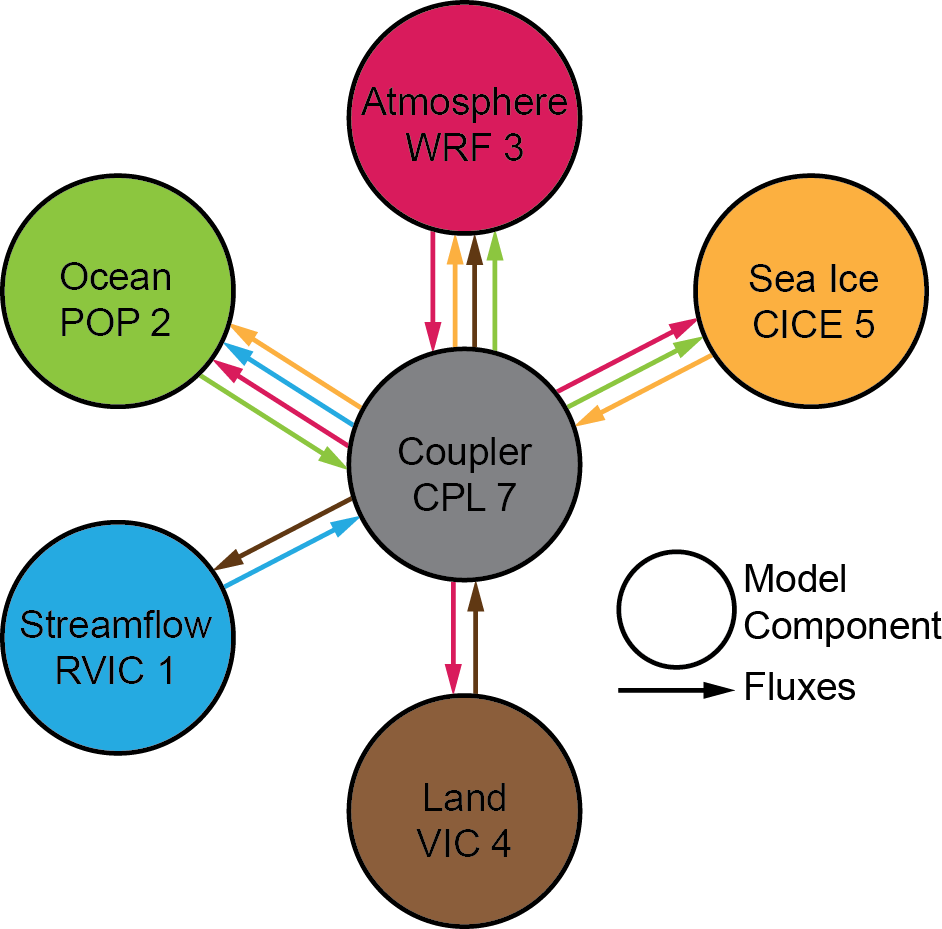
\includegraphics[width=40pc,natwidth=1]{RASM_coupling_schematic}
\caption{Coupling schematic for the Regional Arctic System Model. Circles represent model components (e.g. RVIC) and arrows between circles represent flux and state variables shared between components (e.g. streamflow). The colors of the arrows reflect the source of the fluxes and state variables.}
\label{fig:rasm_coupling_schematic}
\end{figure}

\clearpage
\begin{figure}
\noindent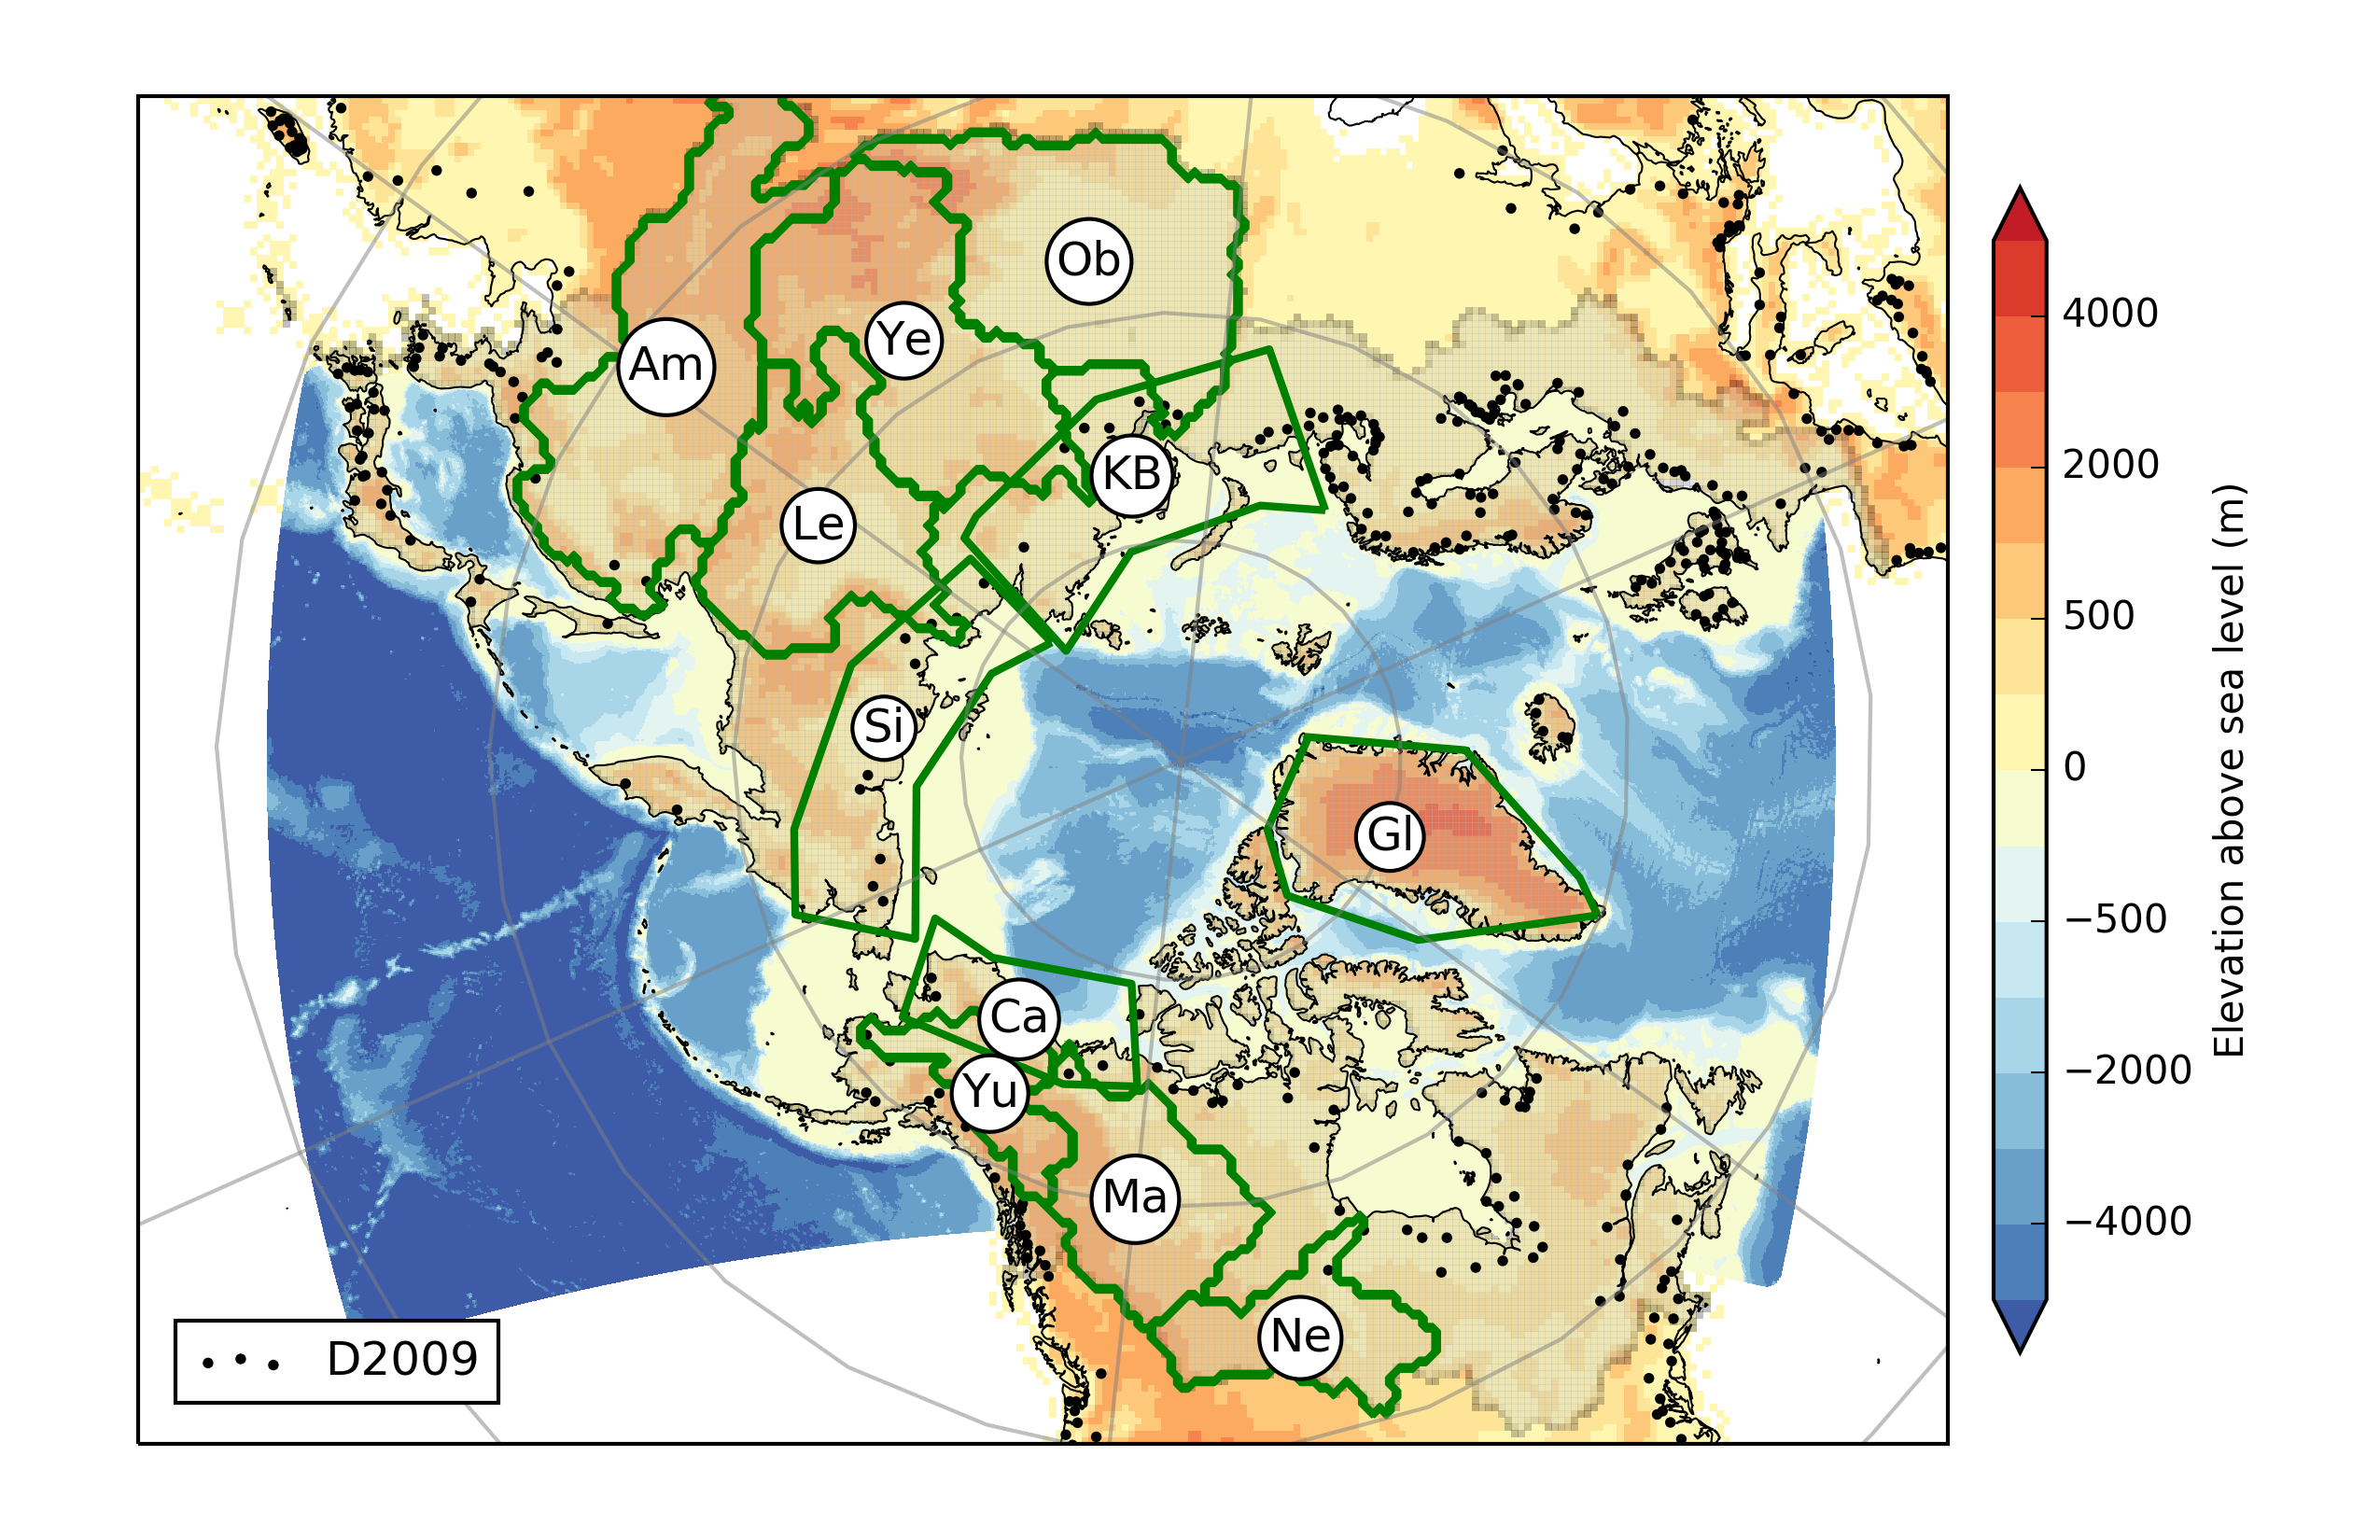
\includegraphics[width=40pc,natwidth=1]{RASM_domain_fig}
\caption{The Regional Arctic System Model domain, showing the 50-km near equal area domain shared by the land, atmosphere, and streamflow routing components (outer rectangle), and the 1/12$^\circ$ ocean-sea ice domain (blue shading).
The RVIC drainage area is highlighted with gray shading and the central Arctic Ocean basin is outlined in gray (Ca).
The seven largest river basins in the RASM domain are outlined in green: Amur (Am), Ob' (Ob), Yenisey (Ye), Lena (Le), Mackenzie (Ma), Nelson (Ne), and Yukon (Yu).
The coastal streamflow flux masks used in section \ref{sec:results} are outlined in blue: Canadian Coast (Ca), Siberian Coast (Si), Kara and Barents Coast (KB), and Greenland (Gl).
The location of the streamflow observations from $D2009$ are shown with red circles.}
\label{fig:rasm_domain}
\end{figure}

\clearpage
\begin{figure}
\noindent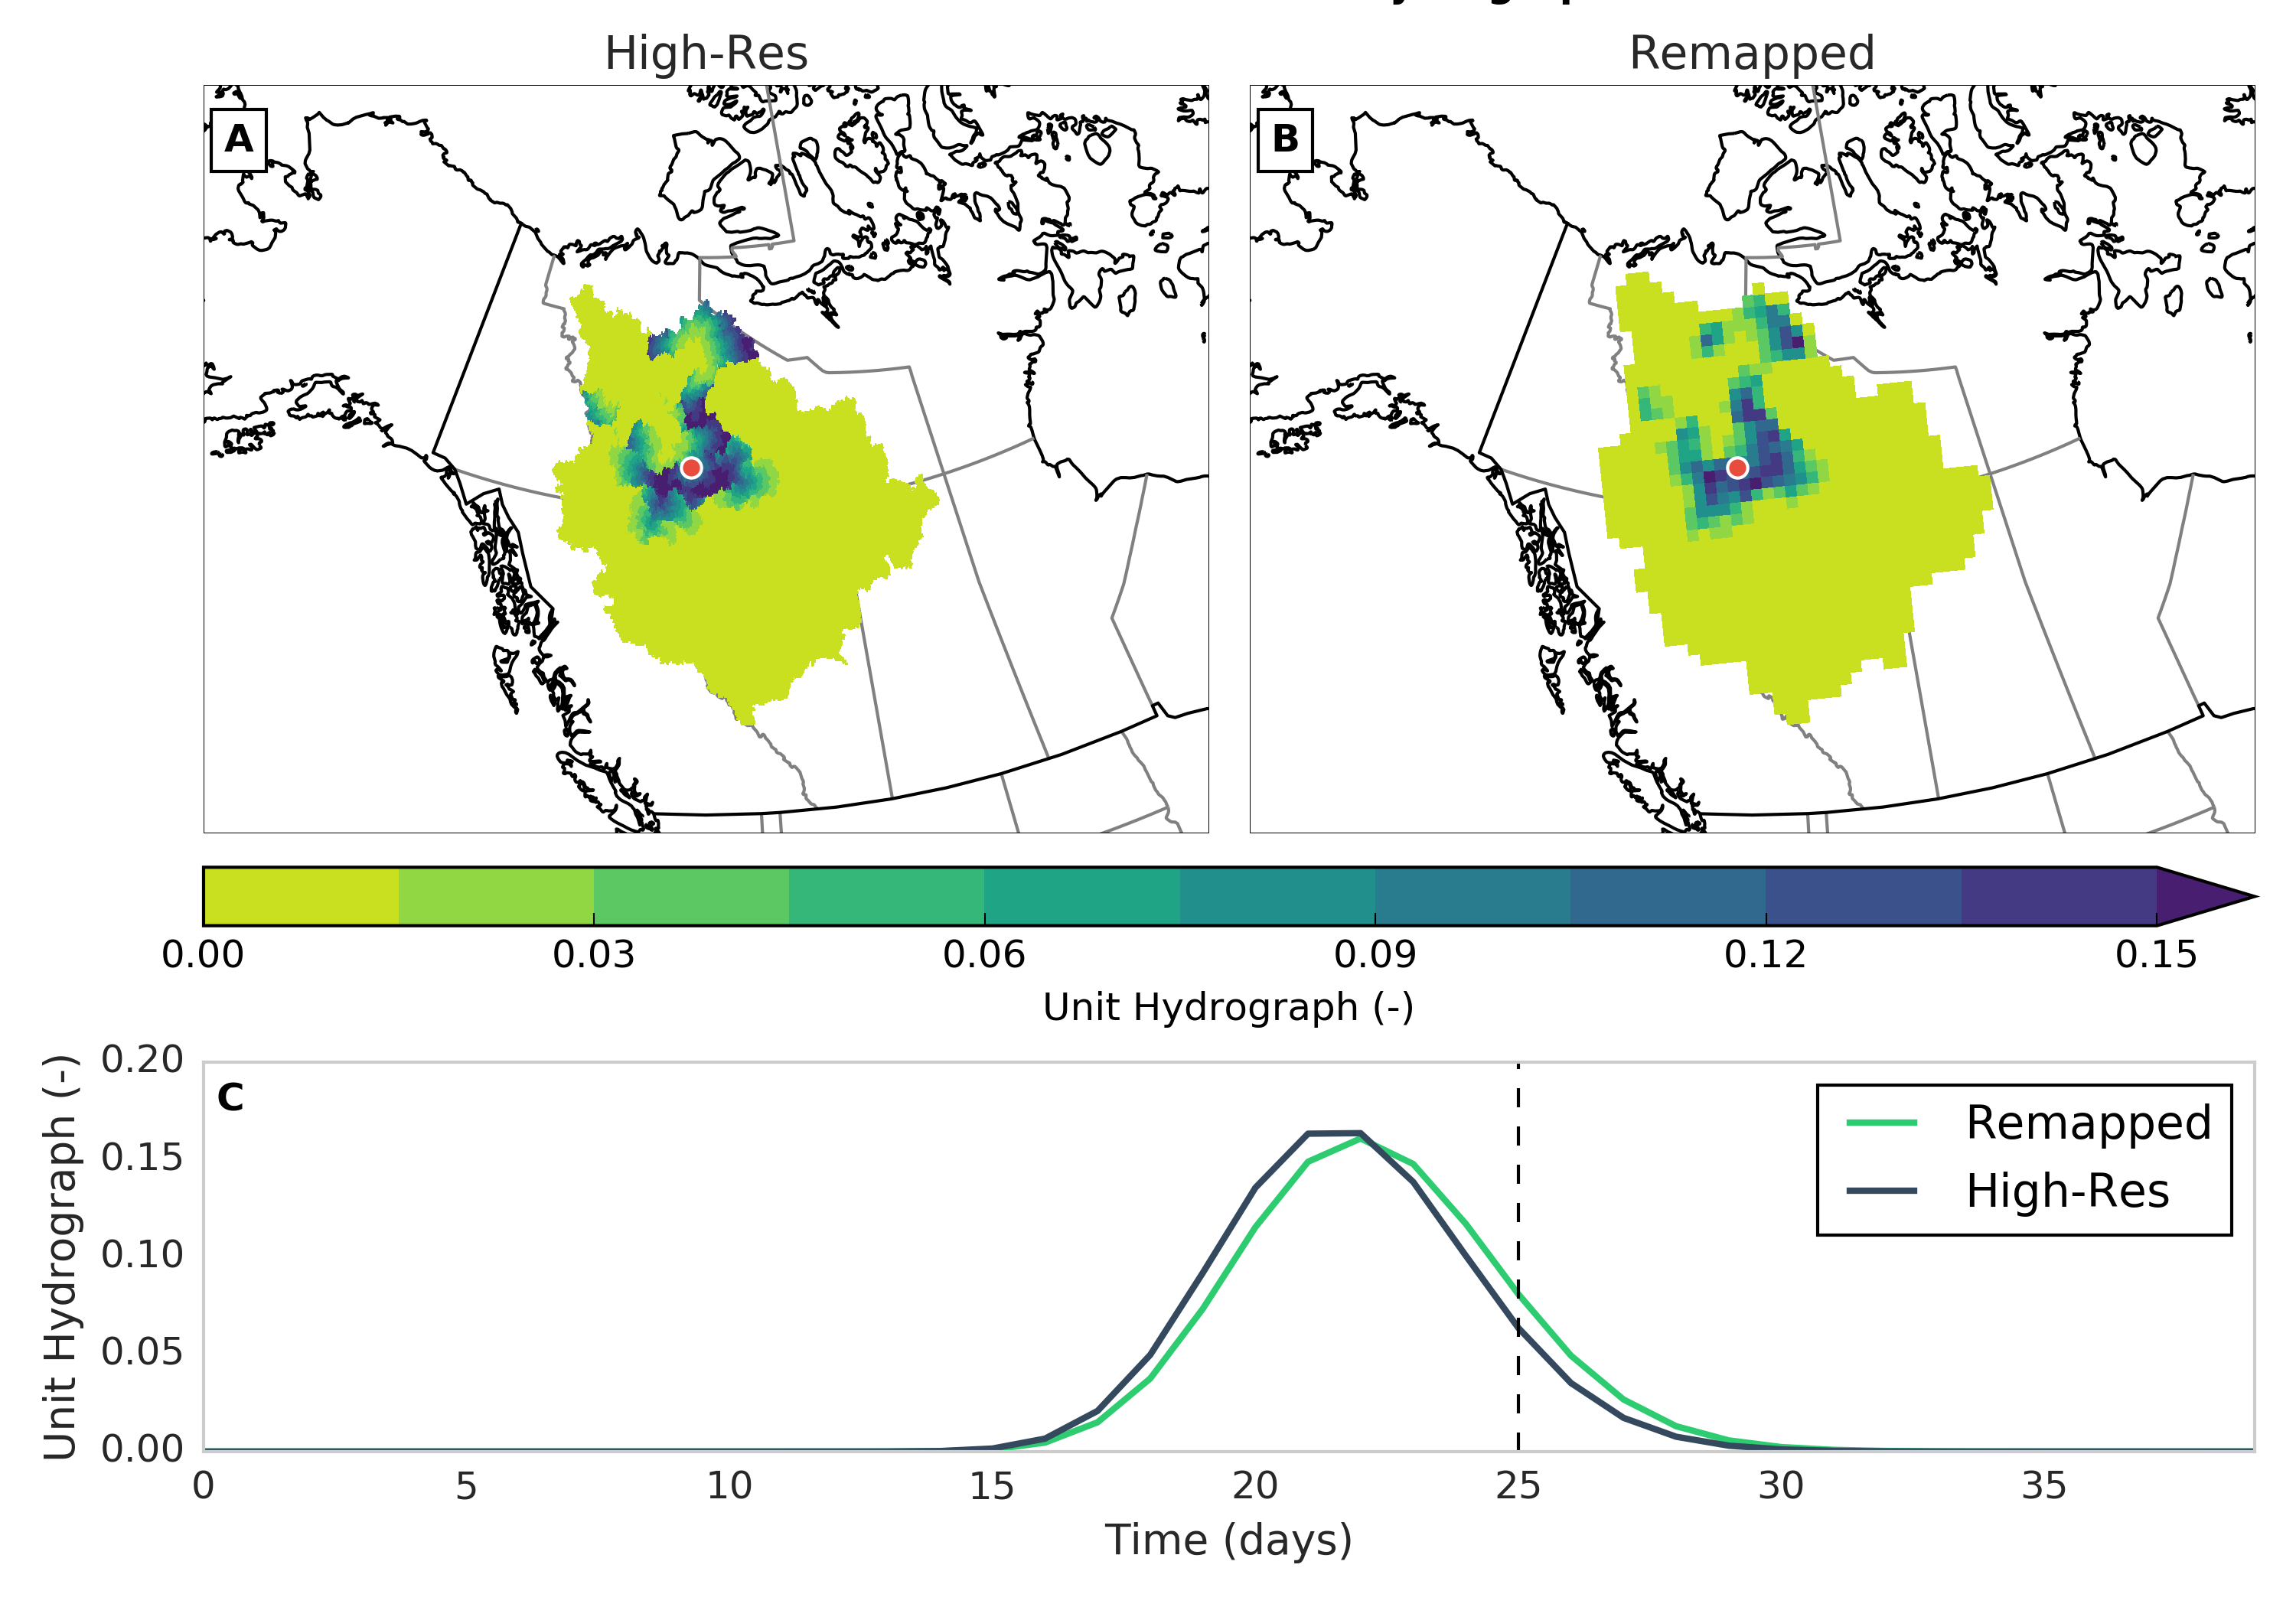
\includegraphics[width=40pc,natwidth=1]{uh_remap_schematic}
\caption{Top: High-resolution (A) and remapped (B) IRFs for the Mackenzie River upstream of the Arctic Red River observation location for timestep 25.
Bottom: IRFs from the high-resolution (blue) and remapped (green) grids at the example location (61.62$^\circ$N, 121.16$^\circ$W) shown in A and B.
The offset between the two IRFs shown in C is the result of spatial averaging during the remapping step.}
\label{fig:uh_remap_schematic}
\end{figure}

\clearpage
\begin{figure}
\noindent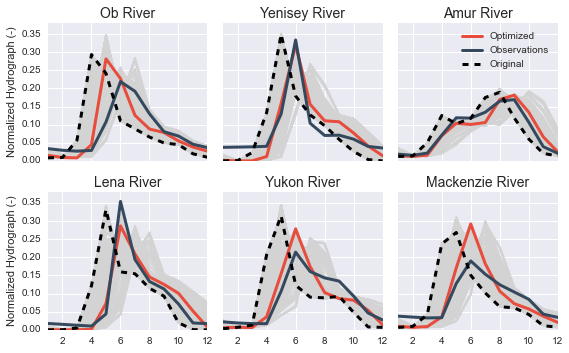
\includegraphics[width=35pc,natwidth=1]{calibration_hydrographs}
\caption{Normalized annual hydrographs for largest six river basins in the RASM domain.
Each trace (grey) represents an individual calibration ensemble member.
The hydrographs using the optimized parameters are shown with blue lines.
The normalized observed hydrograph from $D2009$ for each basin is shown with the dashed black line and the hydrograph using the $RVIC_{FAST}$ (default) parameters is shown with the red line.}
\label{fig:calibration_hydrographs}
\end{figure}

\clearpage
\begin{figure}
\noindent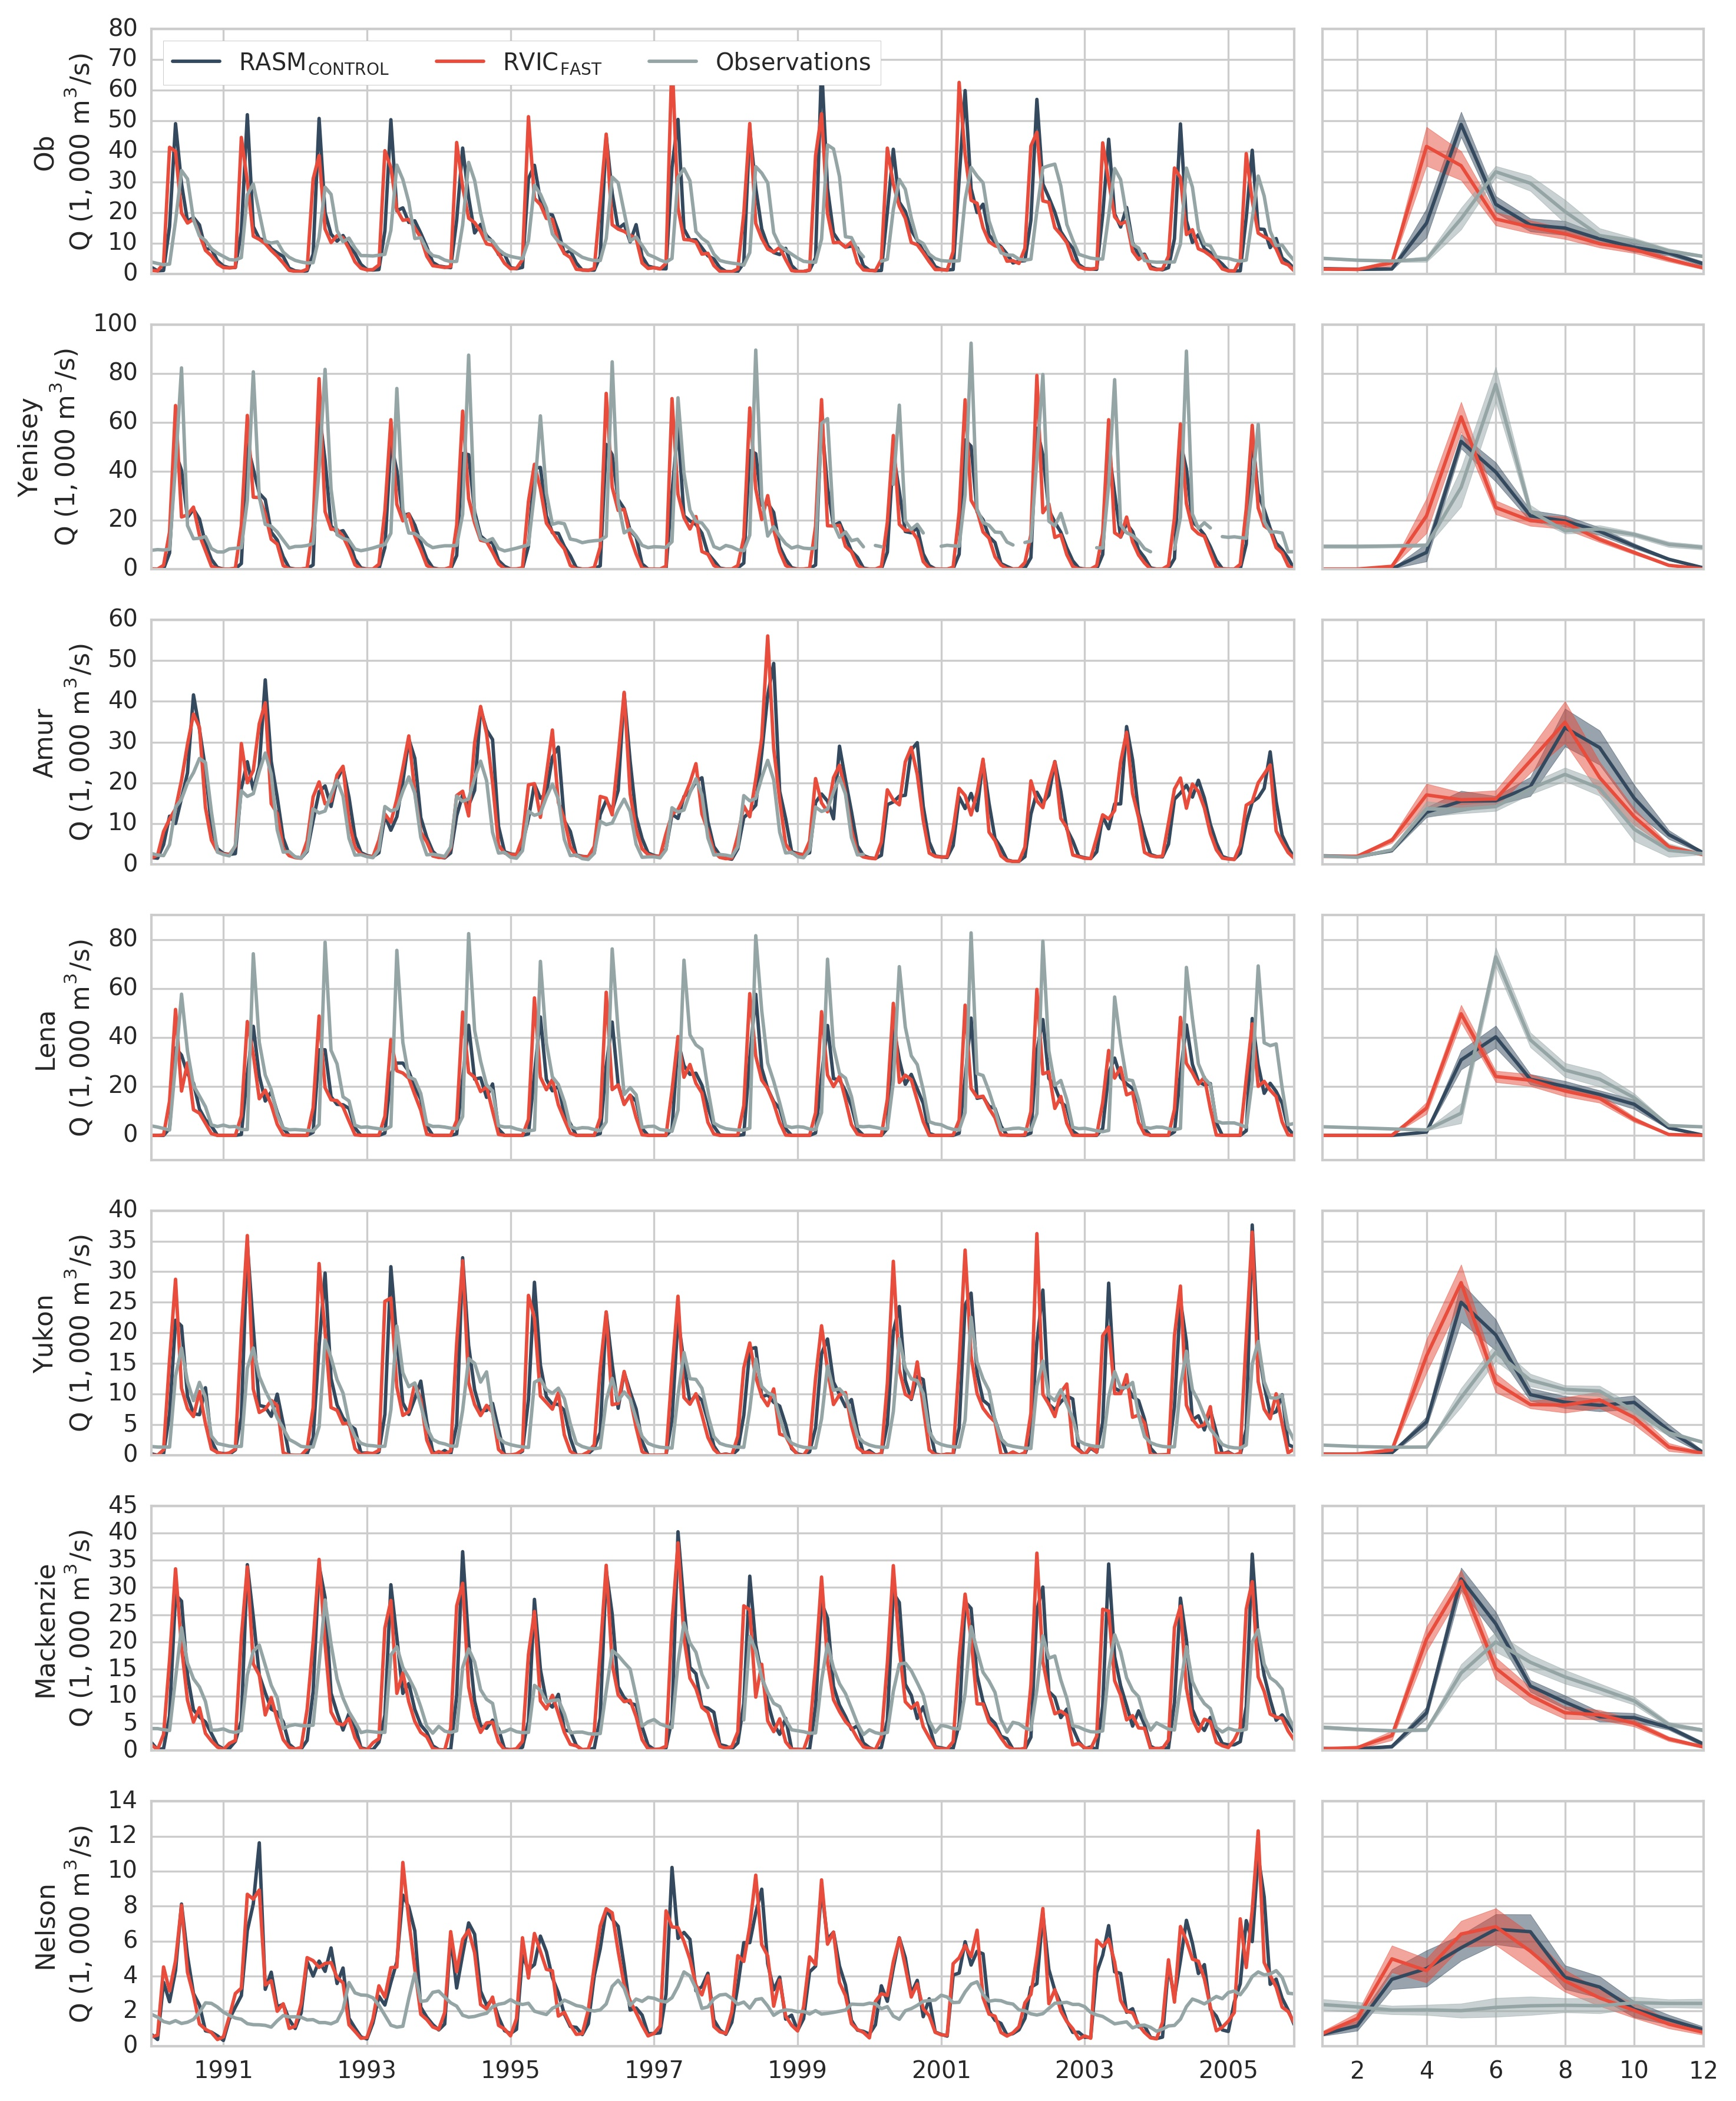
\includegraphics[width=35pc,natwidth=1]{R1010RBRbaaa01a_rvicfast_hydrographs}
\caption{Streamflow hydrographs from $RASM_{CONTROL}$ (blue) and $RVIC_{FAST}$ (red) for the largest seven river basins compared to values from $D2009$ (gray).
The left column includes the monthly streamflow timeseries and the right column includes the monthly mean annual hydrograph where the standard deviation of the interannual variability is represented by the shading.}
\label{fig:hydrographs}
\end{figure}

\clearpage
\begin{figure}
\noindent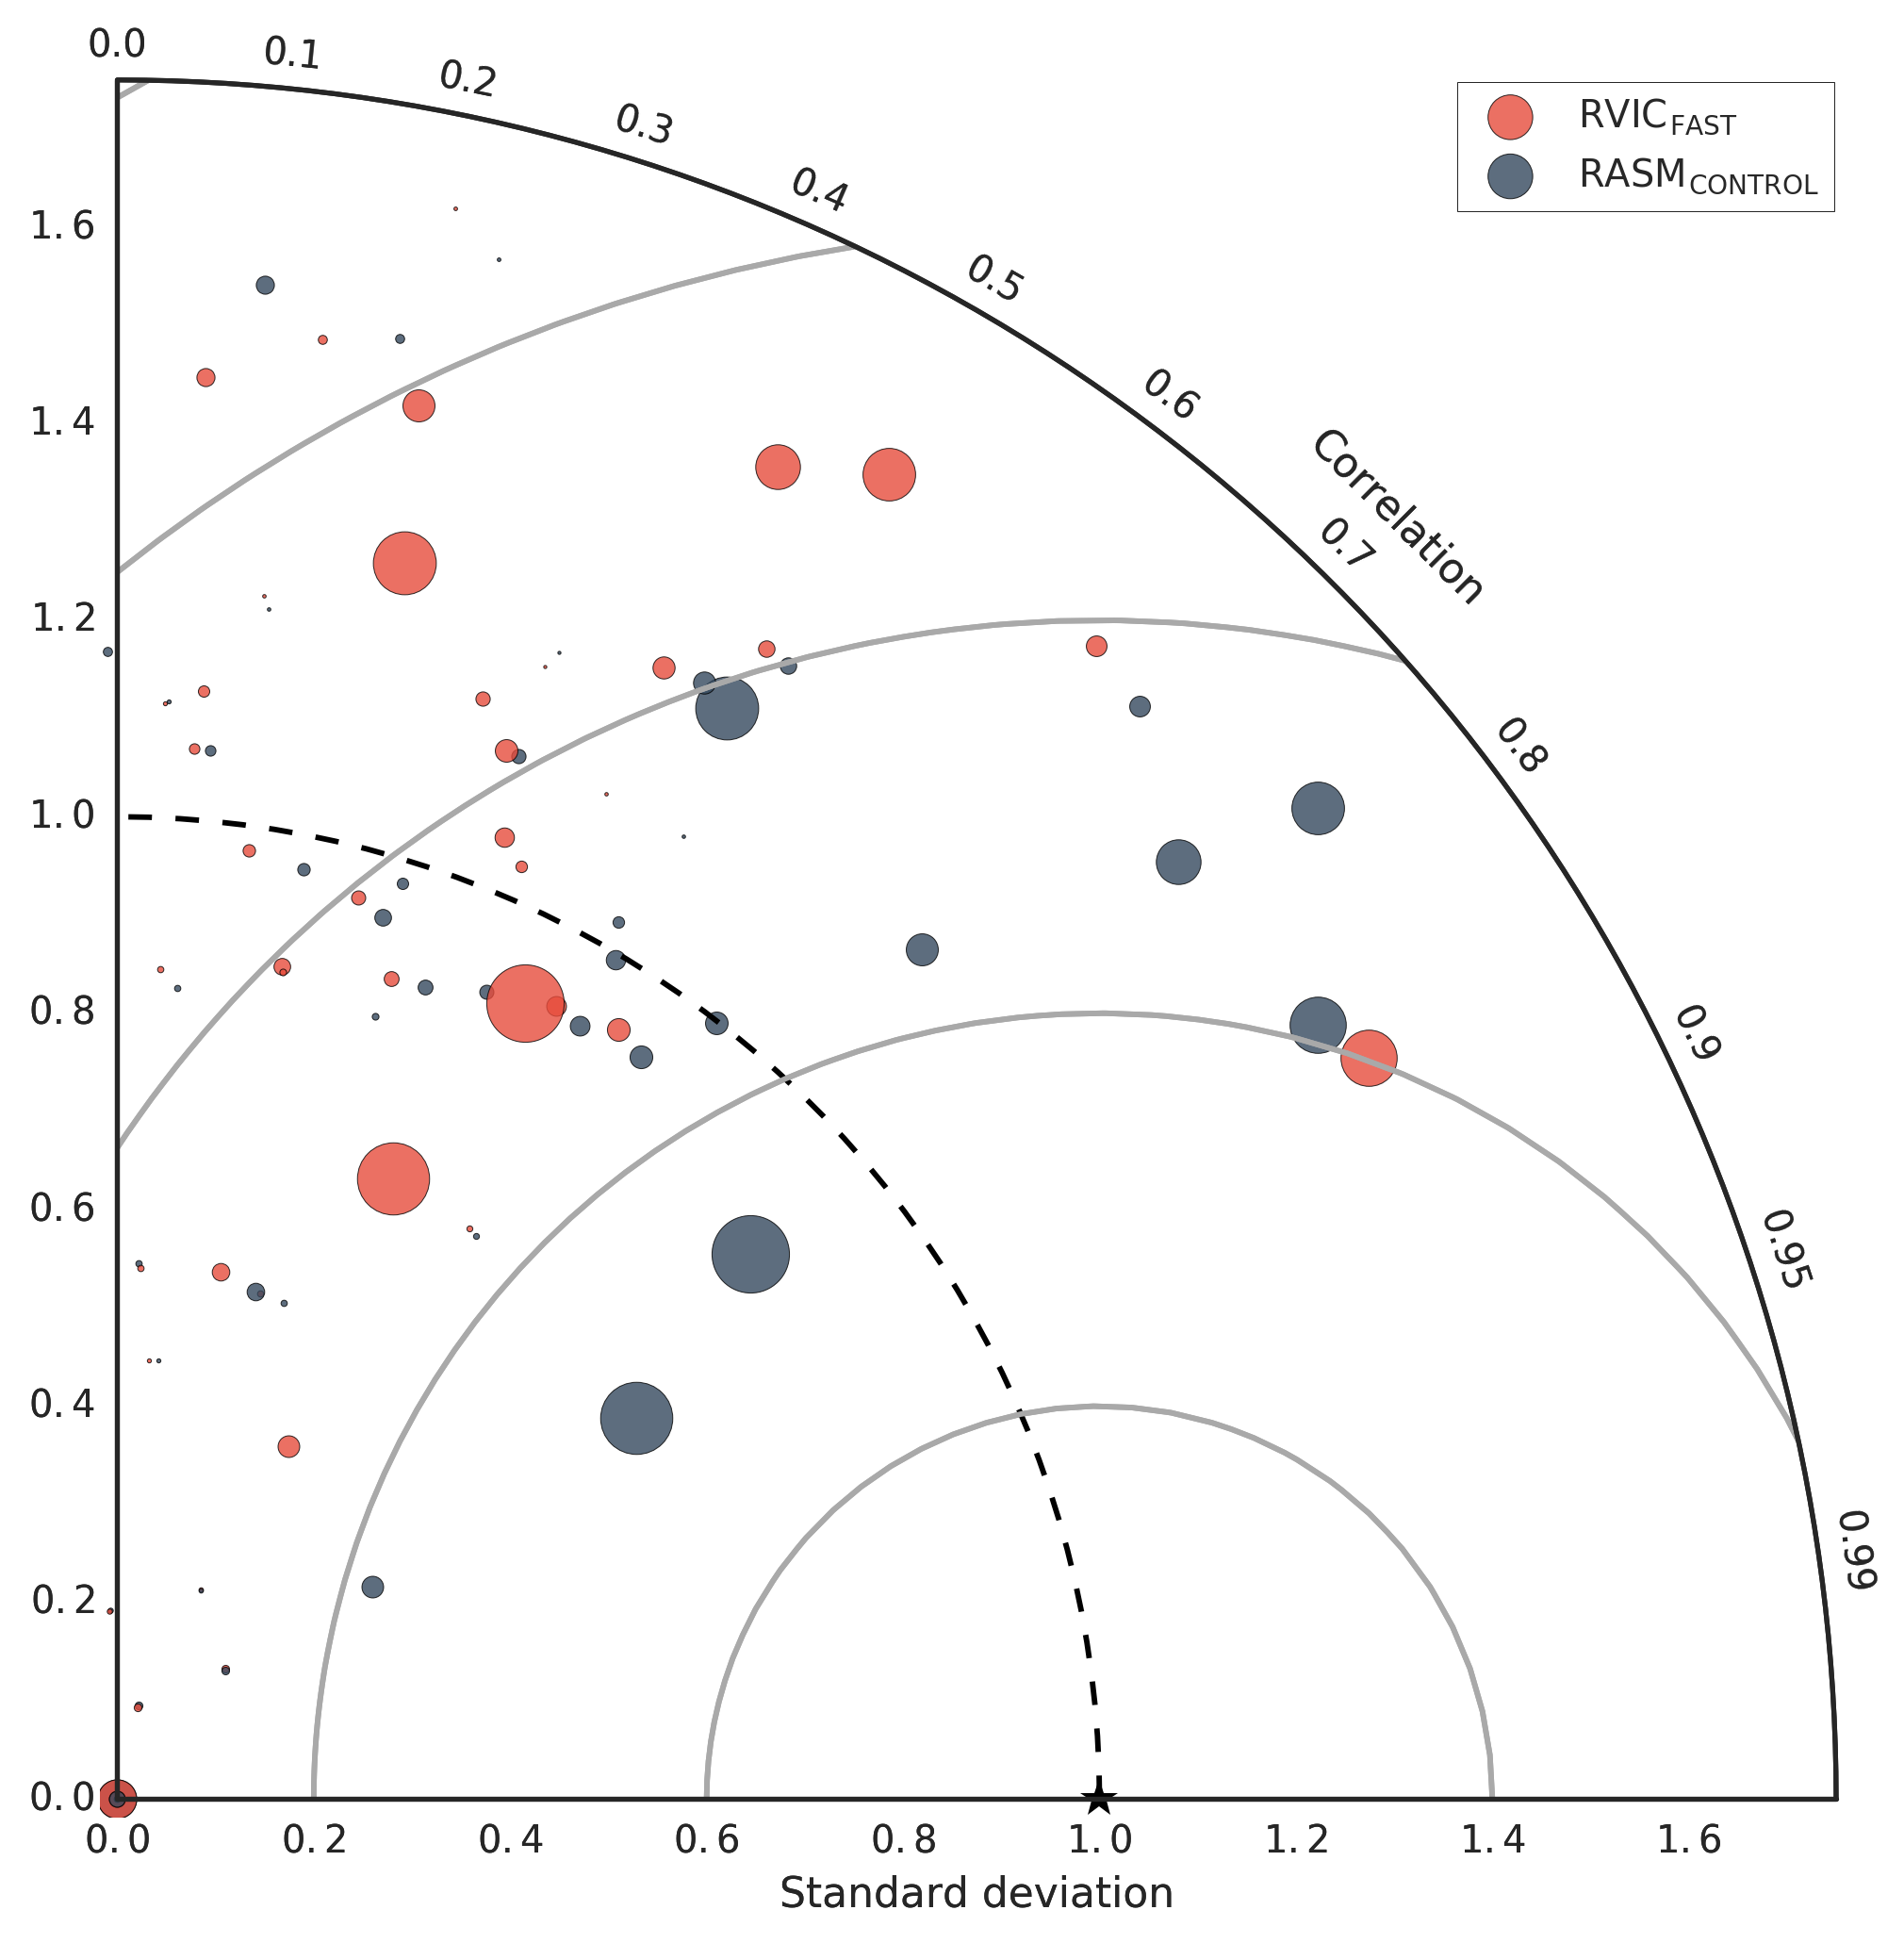
\includegraphics[width=40pc,natwidth=1]{R1010RBRbaaa01a_rvicfast_taylordiag}
\caption{Taylor diagram showing performance of the RVIC model $RASM_{CONTROL}$ (blue) and $RVIC_{FAST}$ (red) for 51 of the largest rivers in the RASM domain.
The reference dataset used as the comparison is $D2009$.
Contours, shown in gray denote constant centered root-mean-squared-differences.
The lines connecting points (only shown for rivers with an annual mean flow greater than 1000 $m^3/s$) represent the change in performance from $RVIC_{FAST}$ to $RASM_{CONTROL}$.
}
\label{fig:taylor}
\end{figure}

\clearpage
\begin{figure}
\noindent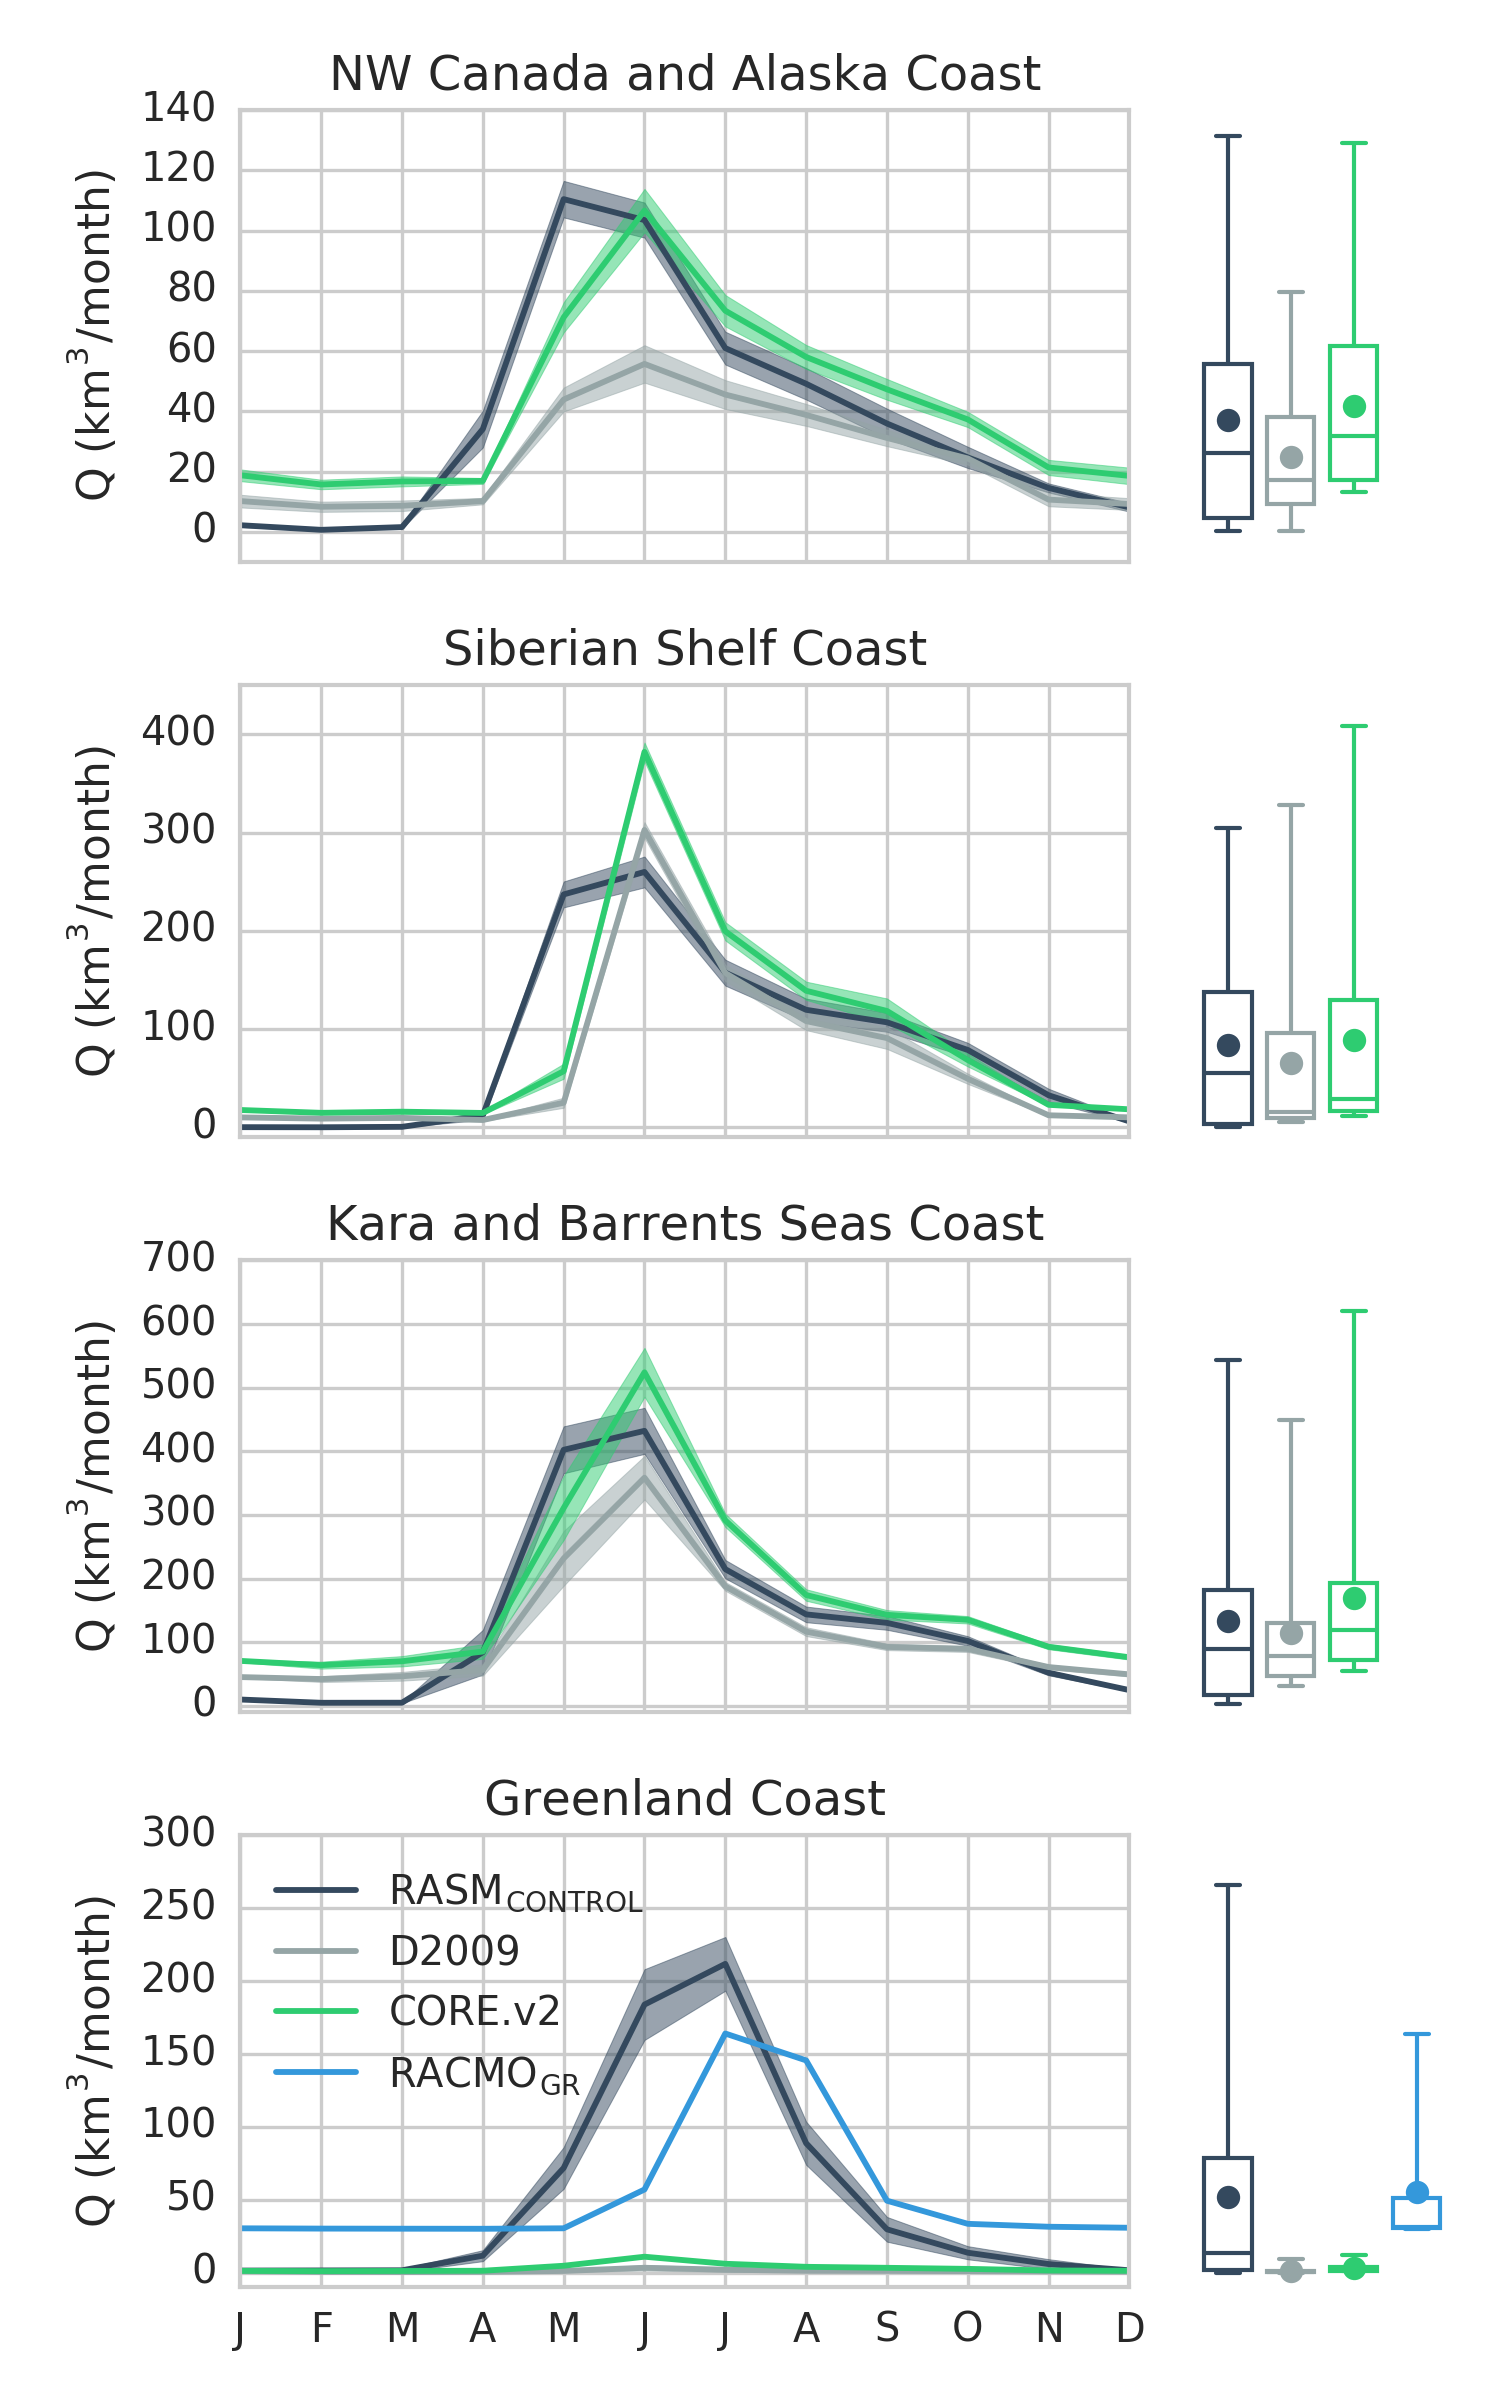
\includegraphics[width=20pc,natwidth=1]{coastal_hydrographs}
\caption{Left: Annual cycle of coastal streamflow fluxes for the four masks shown in Figure \ref{fig:rasm_domain} comparing $RASM_{CONTROL}$ (dark blue), $D2009$ (gray), $CORE.v2$ (green), and $Bamber_{GR}$ (light blue, Greenland only).
Solid lines represent the 1991-1999 mean and the shading denotes the interannual variability.
Right: Box and whisker from the monthly timeseries.
Whiskers represent the full data range, circles represent the mean, horizontal lines represent the median, and the box represents the first and third quartiles.
}
\label{fig:coastal_hydrographs}
\end{figure}


\clearpage
\begin{figure}
\noindent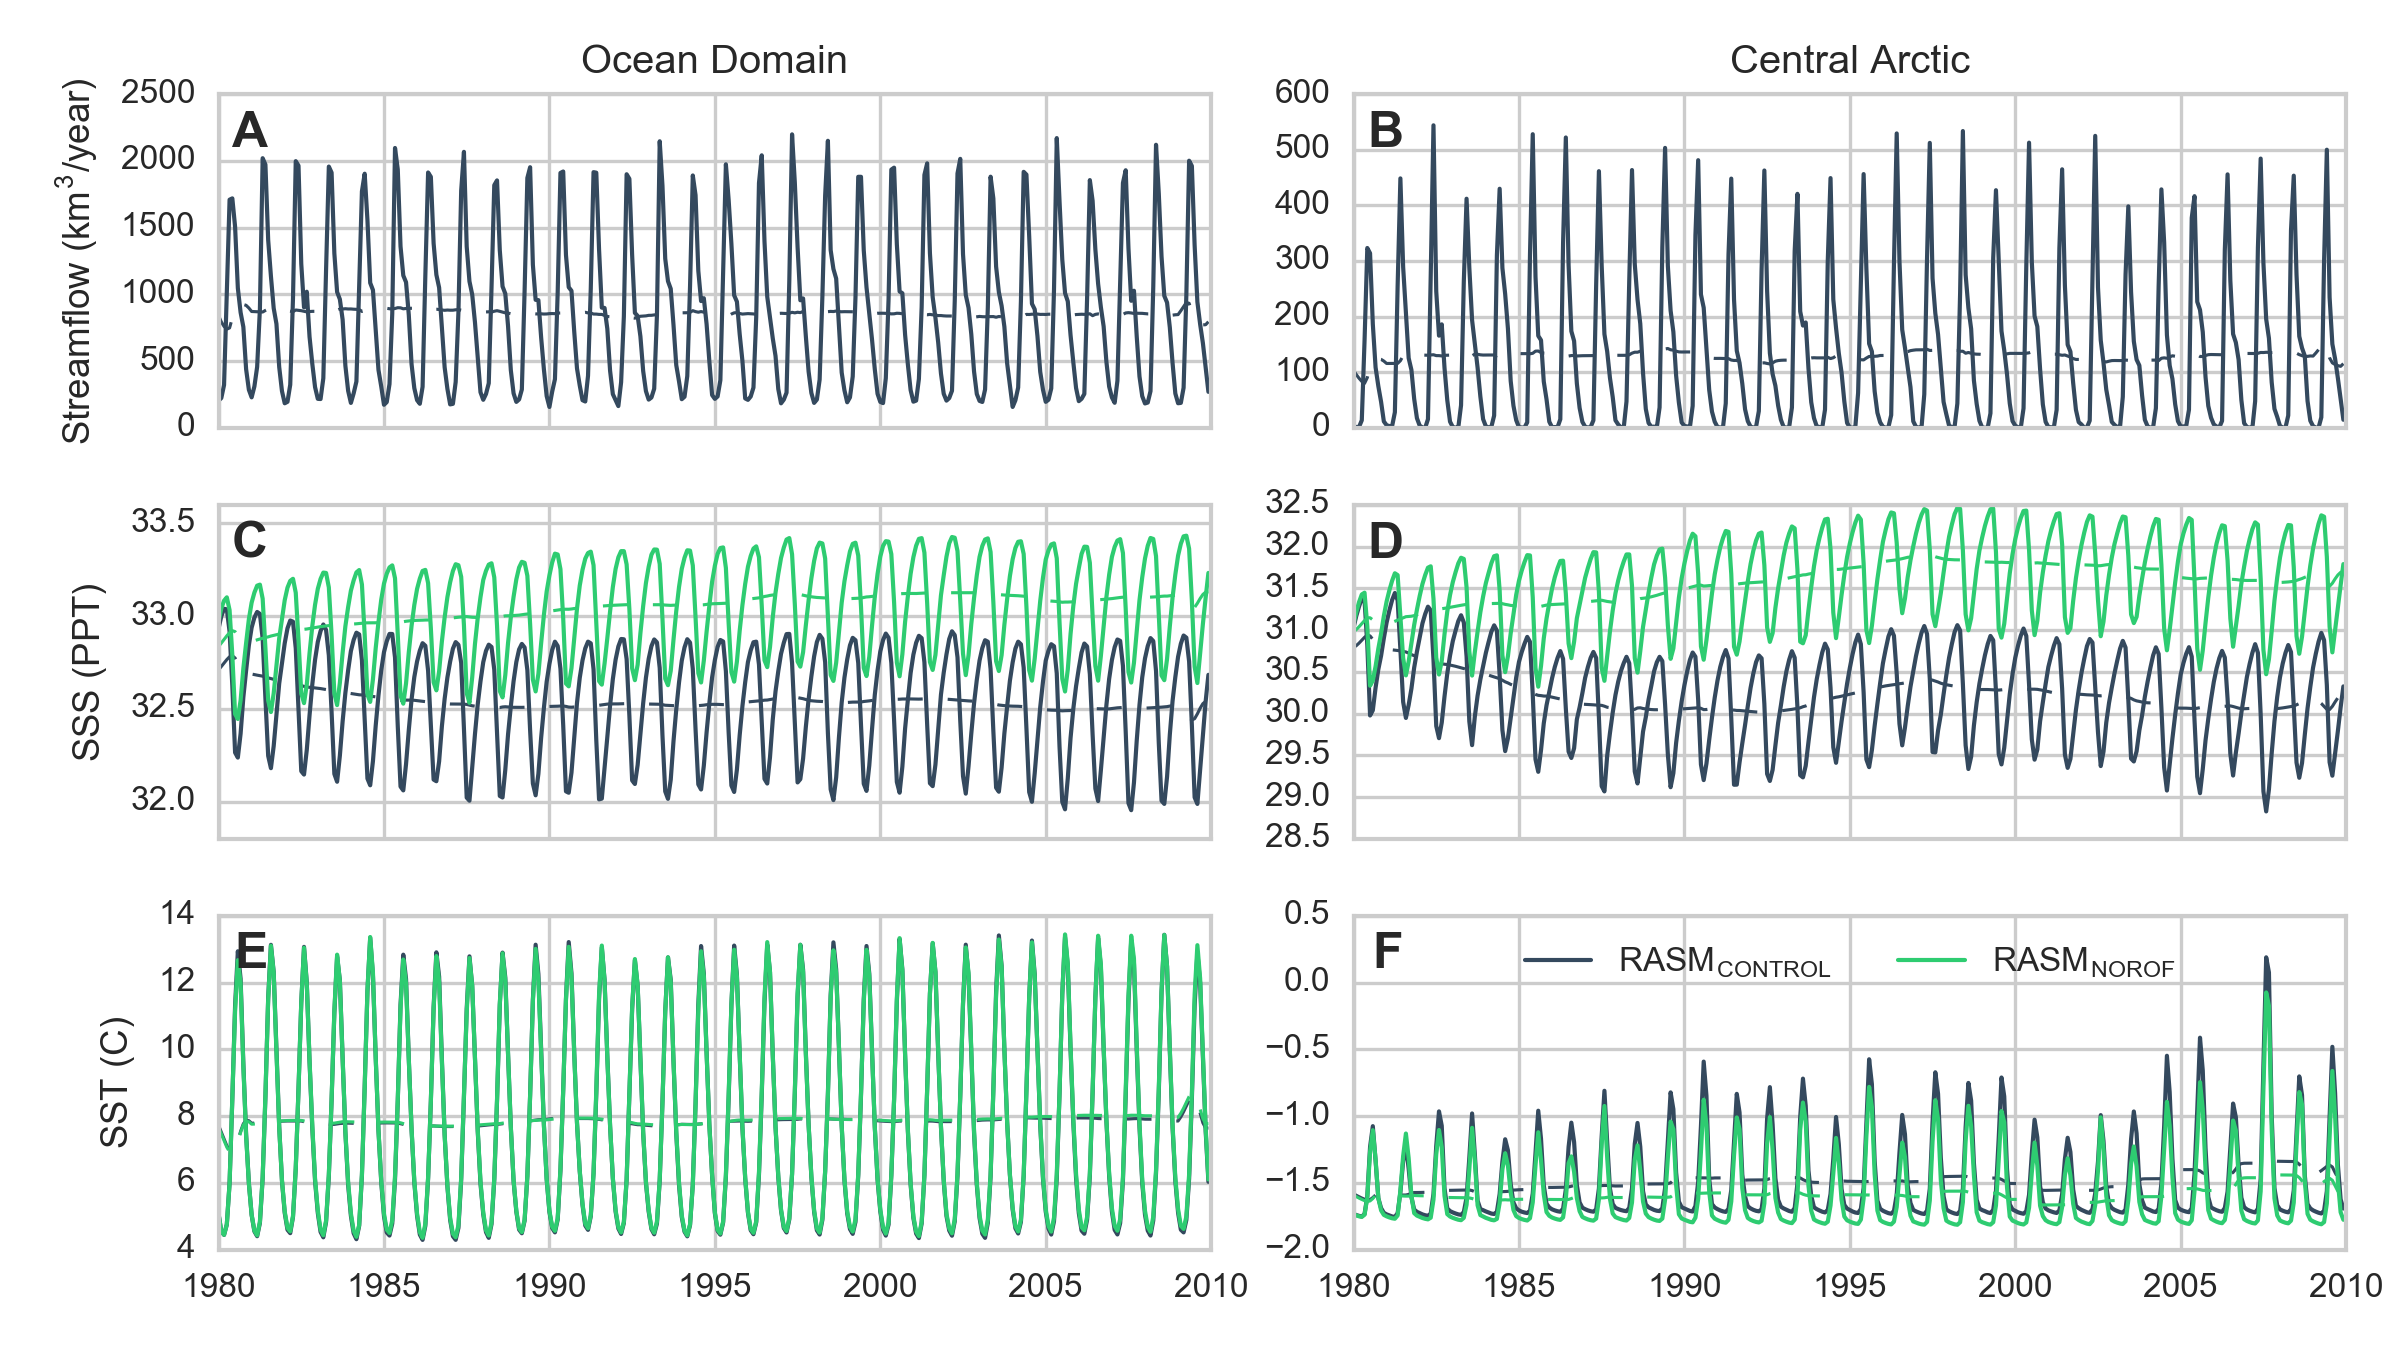
\includegraphics[width=40pc,natwidth=1]{ocean_combine_ts}
\caption{Monthly time series (1980-2009) of domain-wide (left) and central arctic (right) streamflow (top; $RASM_{CONTROL}$ only), mean SSS (middle), and SST (bottom) for the $RASM_{CONTROL}$ (blue) and $RASM_{NOROF}$ (green). The dashed lines show a 12-month running mean.
}
\label{fig:ocean_timeseries}
\end{figure}

\clearpage
\begin{figure}
\noindent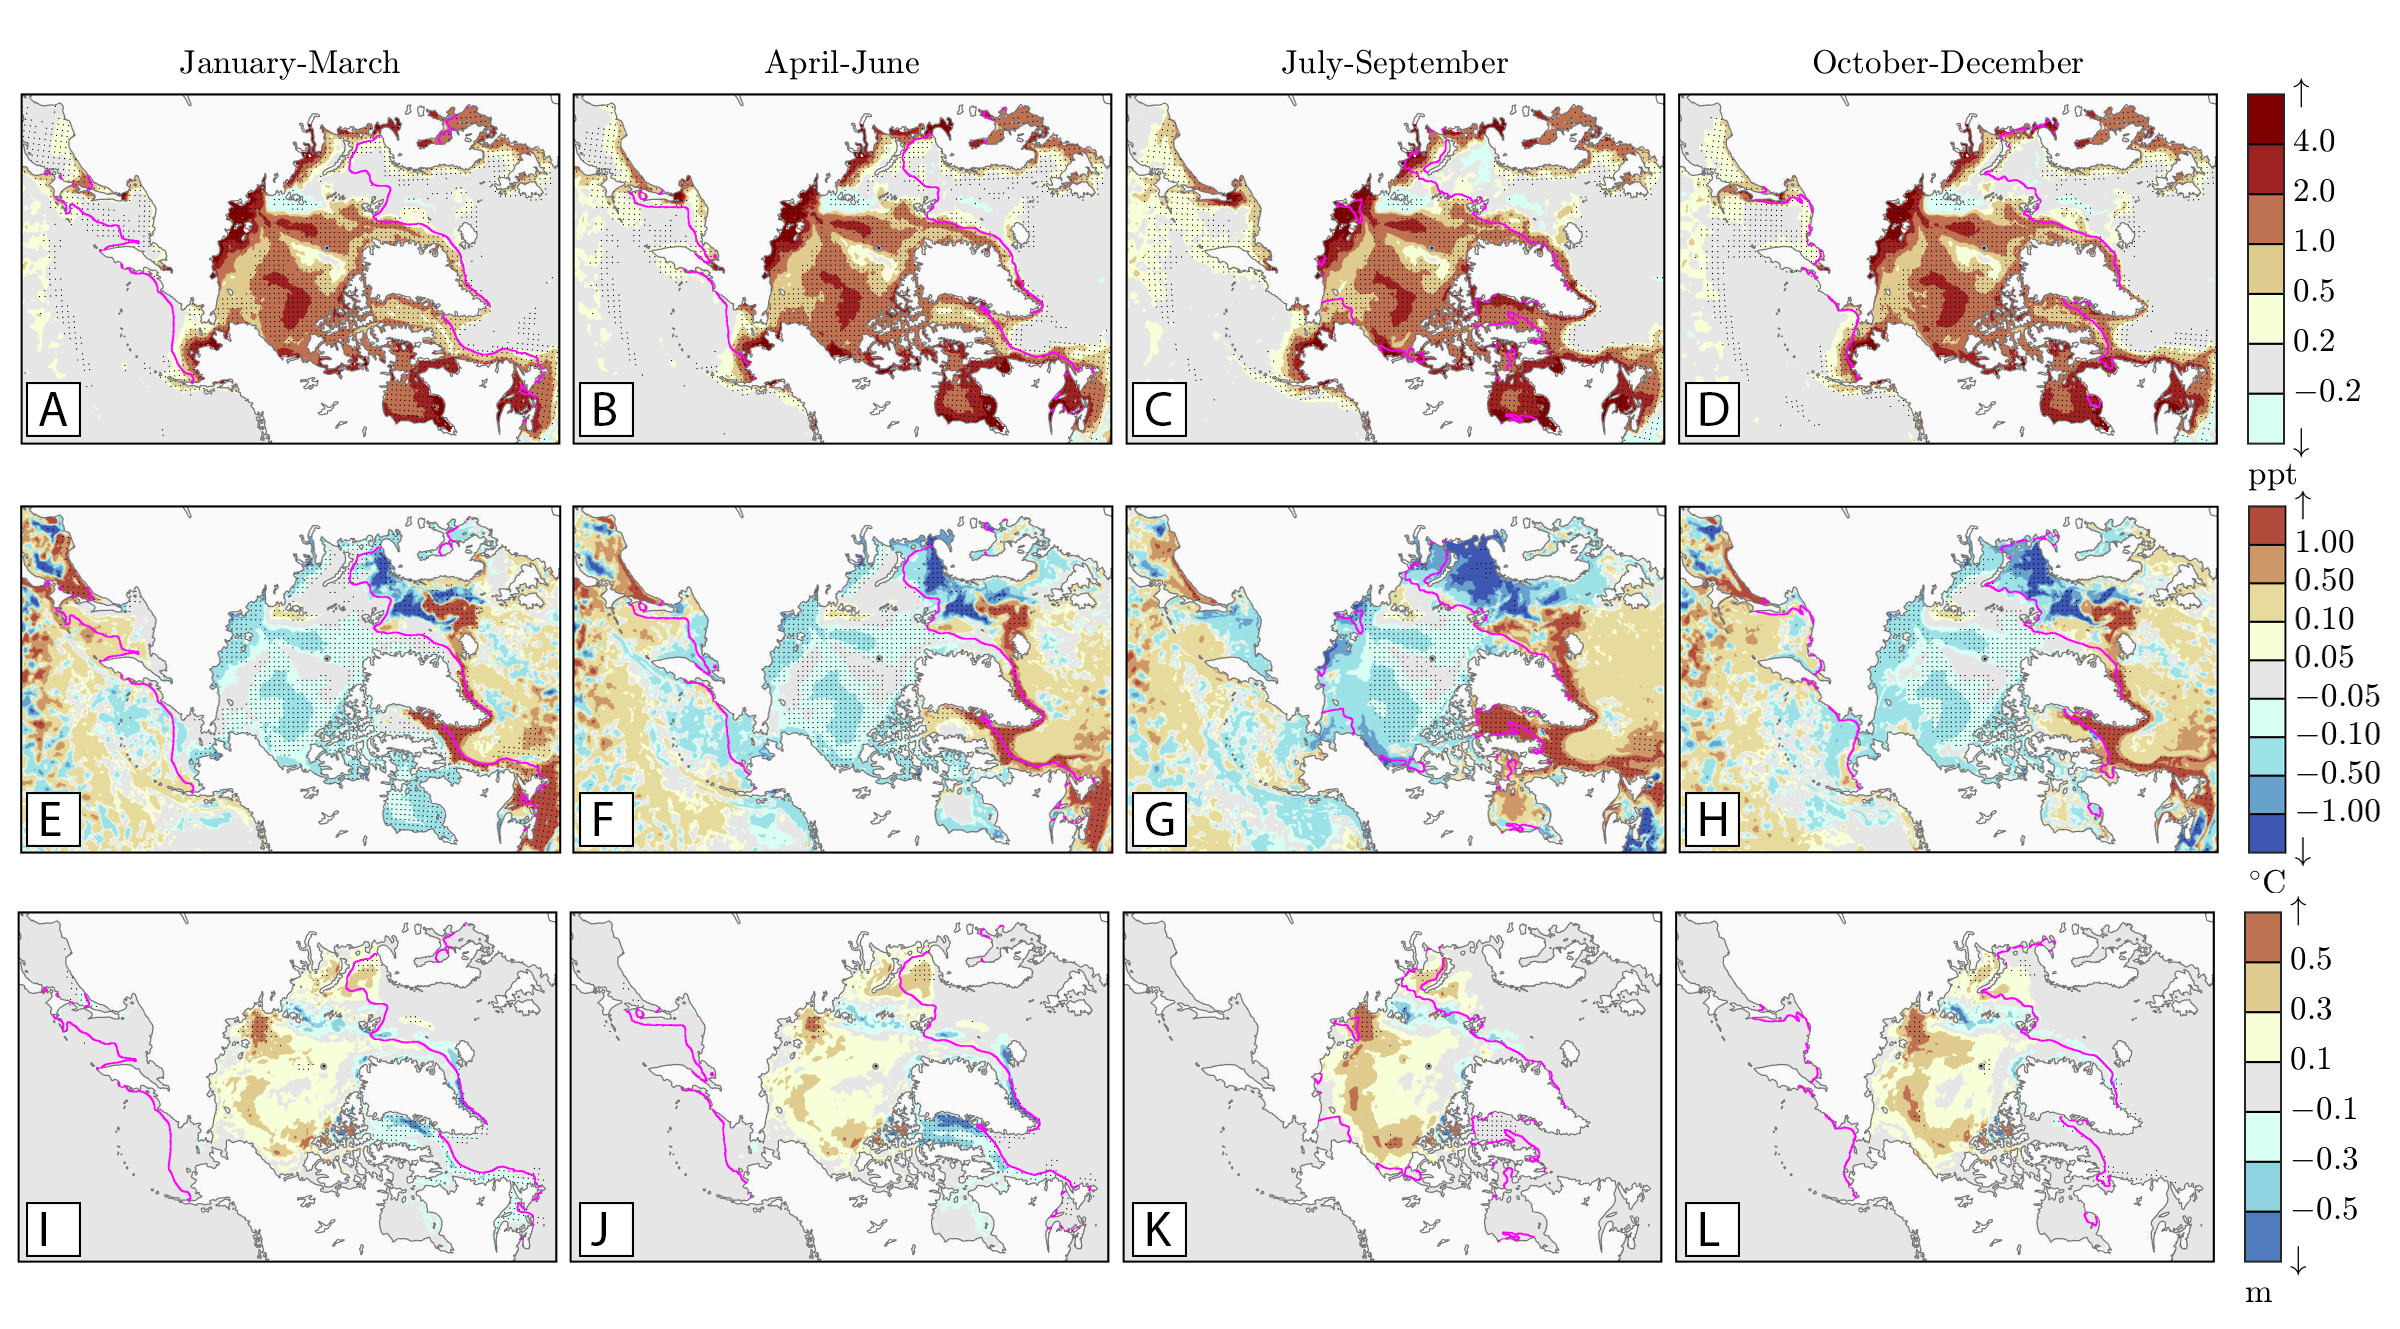
\includegraphics[width=40pc,natwidth=1]{ocean_combine}
\caption{Seasonal difference ($RASM_{NOROF}$ - $RASM_{CONTROL}$) in mean sea surface salinity (top), sea surface temperature (middle), and sea ice thickness (bottom) (2000-2009). Stippling denotes differences that are statistically significant at the 95\%  confidence interval. The magenta contour represents the observed 15\% sea ice concentration contour. }
\label{fig:ocean_maps}
\end{figure}


% Tables
\clearpage

\begin{table}[]
  \caption{Summary of model simulations.}
  \label{table:simulations}
  \begin{tabular}{l|p{4in}}
  Simulation       & Description \\
  $RASM_{CONTROL}$ & Baseline simulation, uses the calibrated RVIC parameters described in section \ref{sec:parameters}. \\
  $RASM_{NOROF}$   & Same as $RASM_{CONTROL}$ except does not include the runoff flux from the land to the ocean. \\
  $RVIC_{FAST}$    & Stand-alone RVIC simulation forced with distributed runoff fields from $RASM_{CONTROL}$. This simulation uses RVIC's default velocity and diffusivity parameters of 2.0 m/s and 2,000 m\textsuperscript{2}/s, respectively.
  \end{tabular}
\end{table}


\begin{table}
  \caption{RVIC model performance statistics for the seven rivers shown in Figure \ref{fig:rasm_domain}. The overlap statistic is calculated using normalized hydrographs whereas the bias and RMSE are calculated using the unadjusted hydrographs.}
  \label{table:rivers}
  \resizebox{\textwidth}{!}{%
  \begin{tabular}{|l|c|c|c|c|c|c|}
  {} & \multicolumn{1}{c}{Bias (\%)} & \multicolumn{2}{c}{Overlap (-)}  &  \multicolumn{2}{c}{RMSE (100 $m^3/s$)} \\
  River                   & $RASM_{CONTROL}$ & $RVIC_{FAST}$ & $RASM_{CONTROL}$ & $RVIC_{FAST}$ & $RASM_{CONTROL}$ \\
  Ob' at Salekhard         &            -3.9  &          0.65 &             0.73 &      148.7    &         120.9    \\
  Yenisey at Igarka       &           -25.8  &          0.64 &             0.75 &      201.1    &         137.9    \\
  Amur at Komsomolsk      &            26.9  &          0.93 &             0.90 &       67.1    &          68.3    \\
  Lena at Kusur           &           -28.0  &          0.64 &             0.80 &      207.3    &         137.1    \\
  Yukon at Pilot          &            13.2  &          0.66 &             0.79 &       73.6    &          50.9    \\
  Mackenzie at Arctic Red &            -4.0  &          0.67 &             0.75 &       82.2    &          62.2    \\
  Nelson at Bladder       &            61.3  &          0.70 &             0.71 &       29.2    &          28.8    \\
  \end{tabular}
}
\end{table}

\end{document}

%%%%%%%%%%%%%%%%%%%%%%%%%%%%%%%%%%%%%%%%%%%%%%%%%%%%%%%%%%%%%%%

More Information and Advice:

%% ------------------------------------------------------------------------ %%
%
%  SECTION HEADS
%
%% ------------------------------------------------------------------------ %%

% Capitalize the first letter of each word (except for
% prepositions, conjunctions, and articles that are
% three or fewer letters).

% AGU follows standard outline style; therefore, there cannot be a section 1 without
% a section 2, or a section 2.3.1 without a section 2.3.2.
% Please make sure your section numbers are balanced.
% ---------------
% Level 1 head
%
% Use the \section{} command to identify level 1 heads;
% type the appropriate head wording between the curly
% brackets, as shown below.
%
%An example:
%\section{Level 1 Head: Introduction}
%
% ---------------
% Level 2 head
%
% Use the \subsection{} command to identify level 2 heads.
%An example:
%\subsection{Level 2 Head}
%
% ---------------
% Level 3 head
%
% Use the \subsubsection{} command to identify level 3 heads
%An example:
%\subsubsection{Level 3 Head}
%
%---------------
% Level 4 head
%
% Use the \subsubsubsection{} command to identify level 3 heads
% An example:
%\subsubsubsection{Level 4 Head} An example.
%
%% ------------------------------------------------------------------------ %%
%
%  IN-TEXT LISTS
%
%% ------------------------------------------------------------------------ %%
%
% Do not use bulleted lists; enumerated lists are okay.
% \begin{enumerate}
% \item
% \item
% \item
% \end{enumerate}
%
%% ------------------------------------------------------------------------ %%
%
%  EQUATIONS
%
%% ------------------------------------------------------------------------ %%

% Single-line equations are centered.
% Equation arrays will appear left-aligned.

Math coded inside display math mode \[ ...\]
 will not be numbered, e.g.,:
 \[ x^2=y^2 + z^2\]

 Math coded inside \begin{equation} and \end{equation} will
 be automatically numbered, e.g.,:
 \begin{equation}
 x^2=y^2 + z^2
 \end{equation}

% IF YOU HAVE MULTI-LINE EQUATIONS, PLEASE
% BREAK THE EQUATIONS INTO TWO OR MORE LINES
% OF SINGLE COLUMN WIDTH (20 pc, 8.3 cm)
% using double backslashes (\\).

% To create multiline equations, use the
% \begin{eqnarray} and \end{eqnarray} environment
% as demonstrated below.
\begin{eqnarray}
  x_{1} & = & (x - x_{0}) \cos \Theta \nonumber \\
        && + (y - y_{0}) \sin \Theta  \nonumber \\
  y_{1} & = & -(x - x_{0}) \sin \Theta \nonumber \\
        && + (y - y_{0}) \cos \Theta.
\end{eqnarray}

%If you don't want an equation number, use the star form:
%\begin{eqnarray*}...\end{eqnarray*}

% Break each line at a sign of operation
% (+, -, etc.) if possible, with the sign of operation
% on the new line.

% Indent second and subsequent lines to align with
% the first character following the equal sign on the
% first line.

% Use an \hspace{} command to insert horizontal space
% into your equation if necessary. Place an appropriate
% unit of measure between the curly braces, e.g.
% \hspace{1in}; you may have to experiment to achieve
% the correct amount of space.


%% ------------------------------------------------------------------------ %%
%
%  EQUATION NUMBERING: COUNTER
%
%% ------------------------------------------------------------------------ %%

% You may change equation numbering by resetting
% the equation counter or by explicitly numbering
% an equation.

% To explicitly number an equation, type \eqnum{}
% (with the desired number between the brackets)
% after the \begin{equation} or \begin{eqnarray}
% command.  The \eqnum{} command will affect only
% the equation it appears with; LaTeX will number
% any equations appearing later in the manuscript
% according to the equation counter.
%

% If you have a multiline equation that needs only
% one equation number, use a \nonumber command in
% front of the double backslashes (\\) as shown in
% the multiline equation above.

%% ------------------------------------------------------------------------ %%
%
%  SIDEWAYS FIGURE AND TABLE EXAMPLES
%
%% ------------------------------------------------------------------------ %%
%
% For tables and figures, add \usepackage{rotating} to the paper and add the rotating.sty file to the folder.
% AGU prefers the use of {sidewaystable} over {landscapetable} as it causes fewer problems.
%
% \begin{sidewaysfigure}
% \includegraphics[width=20pc]{samplefigure.eps}
% \caption{caption here}
% \label{label_here}
% \end{sidewaysfigure}
%
%
%
% \begin{sidewaystable}
% \caption{}
% \begin{tabular}
% Table layout here.
% \end{tabular}
% \end{sidewaystable}
%
